\documentclass[aspectratio=169]{beamer}
\PassOptionsToPackage{CJKpunct=false}{xeCJK}

\usepackage{xcolor}
\newcommand{\cmark}{\textcolor{green!60!black}{$\checkmark$}}
\newcommand{\xmark}{\textcolor{red!70!black}{$\times$}}

\usepackage[T1]{fontenc}
\usepackage[utf8]{inputenc}

\usetheme{BFHhust}

\usepackage{color}
\usepackage{hyperref}
\usepackage{ragged2e}
\usepackage{mathrsfs}
\usepackage{graphicx}
\usepackage{scalerel}
\usepackage{xspace}
\usepackage{tabularx}
\usepackage{amssymb}
\usepackage{multirow}
\usepackage{makecell}
\usepackage{enumitem}
\usepackage{booktabs}
\usepackage{caption}
\usepackage{subcaption}
\usepackage{amsmath,bm,mathtools,times}

\newcolumntype{Y}{>{\centering\arraybackslash}X}
\newcolumntype{L}{>{\raggedright\arraybackslash}X}

% Math operators
\DeclareMathOperator*{\argmax}{argmax}
\DeclareMathOperator*{\argmin}{argmin}

% Crypto shorthand
\newcommand{\Adv}{\mathsf{Adv}}
\newcommand{\msf}[1]{\mathsf{#1}}
\newcommand{\calA}{\mathcal{A}}
\newcommand{\calS}{\mathcal{S}}
\newcommand{\calG}{\mathcal{G}}
\newcommand{\bbG}{\mathbb{G}}
\newcommand{\TSet}{\mathsf{TSet}}
\newcommand{\XSet}{\mathsf{XSet}}
\newcommand{\OPRF}{\mathsf{OPRF}}

\usepackage{pgfpages}
\usetikzlibrary{arrows.meta,positioning,shadows.blur}

% ---- TITLE INFO ----
\titlegraphic{
\includegraphics[scale=0.09]{./float/hust-logo.png}}
\title{面向多用户多关键词的\\可验证可搜索加密方案研究}
\author[张柏川]{答辩人：张柏川 \quad 指导教师：王婧~副教授}
\date{2026 年 4 月}
\institute[HUST]{
  {\fontsize{9pt}{12pt}\selectfont 网络空间安全学院\\}
  \vspace{0.5em}
  {\fontsize{10pt}{12pt}\selectfont 华中科技大学}
}

\begin{document}

\maketitle

% ---- 目录 ----
\begin{frame}{目\quad 录}
  \tableofcontents
\end{frame}

% ============================================================
%  第一章：研究背景与意义
% ============================================================
\section{研究背景与意义}

% ---- Slide: 研究背景 ----
\begin{frame}{研究背景}

  \begin{columns}[T]
    \column{0.55\textwidth}
      \textbf{云存储的安全挑战}
      \begin{itemize}
        \item 数据规模持续增长，敏感信息大量上云
        \item 外部渗透、内部越权、服务商窥探等多重威胁
        \item 传统加密存储使明文检索能力\textbf{完全丧失}
      \end{itemize}

      \vspace{0.8em}
      \textbf{可搜索加密（SSE）的核心价值}
      \begin{itemize}
        \item 在密文上直接执行关键词检索
        \item 实现\textbf{数据隐私}与\textbf{检索可用性}的平衡
        \item 演进路径：单关键词 $\to$ 合取查询 $\to$ 动态更新 $\to$ 多用户
      \end{itemize}

    \column{0.42\textwidth}
      \begin{block}{典型三方架构}
        \begin{center}
          \begin{tabular}{c}
            \textbf{授权管理方 $\mathcal{G}$}\\
            \small 持主密钥，负责令牌签发\\[0.6em]
            $\updownarrow$\\[0.4em]
            \textbf{授权用户 $\mathcal{C}_i$}\\
            \small 发起查询，验证结果\\[0.6em]
            $\updownarrow$\\[0.4em]
            \textbf{云服务器 $\mathcal{S}$}\\
            \small 存储加密索引，执行检索
          \end{tabular}
        \end{center}
      \end{block}
  \end{columns}

\end{frame}

% ---- Slide: 核心问题与挑战 ----
\begin{frame}{核心问题与挑战}

  \begin{alertblock}{根本矛盾}
    恶意云服务器可能\textbf{偏离协议执行}，返回不完整或伪造的搜索结果，
    而授权用户\textbf{缺乏有效验证手段}。
  \end{alertblock}

  \vspace{0.5em}

  \begin{columns}[T]
    \column{0.32\textwidth}
      \begin{block}{(1) 判定位伪造}
        \small
        RBF 资格检验仅输出布尔结果 $\{0,1\}$，
        无密码学凭证，
        恶意方可任意伪造。
      \end{block}
    \column{0.32\textwidth}
      \begin{block}{(2) 地址替换}
        \small
        OPRF 盲化下客户端无法重算物理地址；
        服务器可将采样地址替换为\textbf{未授权位置}，
        绕过资格检验。
      \end{block}
    \column{0.32\textwidth}
      \begin{block}{(3) 版本回放}
        \small
        无版本锚定时，
        服务器可用\textbf{历史状态}应答当前查询，
        静默绕过后续更新。
      \end{block}
  \end{columns}

  \vspace{0.5em}

  \begin{exampleblock}{关键局限}
    现有可验证 SSE 方案大多只验证\textbf{最终结果集}，
    缺乏对检索流程内部——资格检验 / 地址寻址——的系统性验证能力。
  \end{exampleblock}

\end{frame}

% ---- Slide: 研究意义与目标 ----
\begin{frame}{研究意义与本文目标}

  \begin{columns}[T]
    \column{0.48\textwidth}
      \textbf{研究意义}
      \begin{itemize}
        \item \textbf{理论}：将验证粒度从结果集扩展至
              \textbf{位值真实性}与\textbf{地址归属正确性}
        \item \textbf{方法}：在保留 OPRF 盲化与概率数据结构的前提下
              引入密码学承诺层
        \item \textbf{实践}：轻量级附加开销，
              适配多用户云端部署场景
      \end{itemize}

      \vspace{0.8em}
      \textbf{本文贡献（两项核心机制）}
      \begin{itemize}
        \item \textbf{机制一}：基于 Merkle Hash Tree 的可验证
              资格检验机制 $\pi_\mathsf{VQ}$
        \item \textbf{机制二}：基于 Merkle 选择性开封的
              地址绑定验证机制
      \end{itemize}

    \column{0.48\textwidth}
      \begin{exampleblock}{核心目标}
        \centering\large
        把``不可见的内部检索步骤''\\
        转化为\\
        \textbf{具备密码学保障的可验证过程}
      \end{exampleblock}

      \vspace{0.8em}
      \begin{block}{安全假设}
        \begin{itemize}
          \item EUF-CMA 不可伪造签名方案
          \item 抗碰撞哈希函数族
          \item OPRF 伪随机性
        \end{itemize}
      \end{block}
  \end{columns}

\end{frame}

% ============================================================
%  第三章：创新点一——可验证资格检验机制 π_VQ
% ============================================================
\section{创新点一：可验证资格检验机制 $\pi_\mathsf{VQ}$}

% ---- Slide: 研究内容概览 + 系统模型 ----
\begin{frame}{研究内容概览与系统模型}

  \begin{columns}[T]
    \column{0.48\textwidth}
      \begin{exampleblock}{两层轻量级可验证机制}
        \begin{itemize}
          \item \textbf{机制一 $\pi_\mathsf{VQ}$}：\\
                基于 Merkle Hash Tree 的可验证资格检验\\
                \small $\to$ 验证\textbf{位值真实性}
          \vspace{0.3em}
          \item \textbf{机制二}：\\
                基于 Merkle-Open 的地址绑定验证\\
                \small $\to$ 验证\textbf{地址归属正确性}
        \end{itemize}
      \end{exampleblock}

    \column{0.48\textwidth}
      \begin{block}{系统模型（三方）}
        \begin{itemize}
          \item $\mathcal{G}$（授权管理方）：持主密钥，
                版本锚定签发，令牌绑定
          \item $\mathcal{C}_i$（授权用户）：发起查询，
                独立验证服务器响应
          \item $\mathcal{S}$（云服务器）：存储双索引
                $(\TSet, \XSet)$，执行检索与证明生成
        \end{itemize}
      \end{block}
  \end{columns}

  \vspace{0.3em}
  \begin{alertblock}{威胁模型}
    恶意但计算受限的云服务器：
    可偏离协议、可观察泄露信息（搜索/访问/更新模式），
    但\textbf{不能}打破签名不可伪造与哈希抗碰撞。
  \end{alertblock}

\end{frame}

% ---- Slide: π_VQ 动机 ----
\begin{frame}{$\pi_\mathsf{VQ}$ 的设计动机}

  \begin{columns}[T]
    \column{0.48\textwidth}
      \textbf{基础协议的不足}
      \begin{itemize}
        \item 资格检验基于 RBF 概率数据结构
        \item 服务器仅输出布尔判定 $\{0,1\}$
        \item 缺乏密码学验证凭证
        \item 无法区分：
          \begin{itemize}
            \item 真实``未命中''
            \item 恶意服务器伪造的``未命中''
          \end{itemize}
        \item 无版本绑定 $\Rightarrow$ 历史状态回放
      \end{itemize}

    \column{0.48\textwidth}
      \textbf{核心设计思路}
      \begin{itemize}
        \item 在 XSet 位数组 $B^{(t)}$ 上\textbf{叠加承诺层}
        \item 构造 Merkle Hash Tree QTree，不改变 RBF 采样语义
        \item 叶承诺：$L_a^{(t)} = H(0 \,\|\, a \,\|\, B^{(t)}[a])$
        \item 内部节点：$N = H(1 \,\|\, N_\ell \,\|\, N_r)$
        \item 引入\textbf{版本锚定签名}：
              \[\mathsf{Anchor}_t = (t,\; R_X^{(t)},\; \sigma_t)\]
      \end{itemize}
  \end{columns}

\end{frame}

% ---- Slide: π_VQ 构造与证据类型 ----
\begin{frame}{$\pi_\mathsf{VQ}$ 构造：四个关键算法}

  \begin{columns}[T]
    \column{0.50\textwidth}
      \begin{block}{\textsc{Commit}（授权管理方）}
        \small
        对完整位数组 $B^{(t)}$ 构建 QTree；\\
        初始化 $O(M)$ 哈希，更新仅需 $O(\ell \log M)$ 增量。
      \end{block}

      \begin{block}{\textsc{TokenBind}（授权管理方）}
        \small
        令牌附加版本号 $t$ 与采样索引 $\nu$，\\
        绑定搜索至当前版本状态。
      \end{block}

      \begin{block}{\textsc{Search-Prove}（服务器）}
        \small
        生成 Positive / Negative 两类证据：
        \begin{itemize}
          \item \textbf{Positive}（判定$=1$）：$k$ 条满位地址的认证路径
          \item \textbf{Negative}（判定$=0$）：至少 $1$ 条零位地址反例路径
        \end{itemize}
      \end{block}

    \column{0.48\textwidth}
      \begin{block}{\textsc{Verify}（客户端，三层）}
        \small
        \begin{itemize}
          \item[1.] \textbf{版本校验}：
                $\mathsf{Verify}(\sigma_t,\, t \,\|\, R_X^{(t)}) = 1$
          \item[2.] \textbf{结构校验}：
                每条路径哈希链至根 $R_X^{(t)}$
          \item[3.] \textbf{语义校验}：
                Positive 要求 $k$ 位全为 $1$；\\
                Negative 要求至少 $1$ 位为 $0$
        \end{itemize}
      \end{block}

      \vspace{0.4em}
      \begin{exampleblock}{渐近复杂度}
        \small
        \begin{tabular}{ll}
          \textbf{更新} & $O(\ell \log M)$ 额外哈希 \\
          \textbf{证明生成} & $O((N_+ k + N_-)\log M)$ \\
          \textbf{客户端验证} & $O((N_+ k + N_-)\log M)$ \\
        \end{tabular}
        \vspace{0.2em}\\
        \small $N_+$：正判定数，$N_-$：负判定数
      \end{exampleblock}
  \end{columns}

\end{frame}

% ============================================================
%  第四章：创新点二——地址绑定验证机制
% ============================================================
\section{创新点二：地址绑定验证机制}

% ---- Slide: 地址替换攻击 ----
\begin{frame}{为什么仅有 $\pi_\mathsf{VQ}$ 还不够？}

  \begin{alertblock}{地址替换攻击}
    在 OPRF 盲化架构下，客户端持采样索引 $\nu$ 但\textbf{不掌握} $K_X$，
    无法独立重算物理地址。

    \medskip
    恶意服务器可将采样\textbf{满位地址} $a_0$
    替换为授权集合\textbf{外的零位地址} $a^*$：
    \[
      \mathsf{VfPath}(R_X^{(t)},\; a^*,\; 0,\; \pi_{a^*}) = 1
      \quad\text{仍成立，因为 }a^*\text{ 确实在树中且该位为 }0
    \]

    \textbf{后果}：客户端无法检测替换，文件被错误剔除，可用性受损。
  \end{alertblock}

  \vspace{0.3em}

  \begin{columns}[T]
    \column{0.48\textwidth}
      \begin{block}{设计约束}
        \begin{itemize}
          \item 更新阶段可利用授权方全局视图
          \item 搜索阶段证明开封严格受限于 $k$，不能开封完整 $\ell$ 维集合
          \item 不能泄露未采样位置的地址信息
        \end{itemize}
      \end{block}
    \column{0.48\textwidth}
      \begin{exampleblock}{解决思路：Merkle 选择性开封}
        \begin{itemize}
          \item \textbf{更新}：对完整地址集合建立 Merkle 根承诺
          \item \textbf{搜索}：仅对采样 $k$ 个位置选择性开封
          \item \textbf{验证}：确认采样地址 $\subseteq$ 授权集合
        \end{itemize}
      \end{exampleblock}
  \end{columns}

\end{frame}

% ---- Slide: Merkle-Open 构造 ----
\begin{frame}{Merkle-Open 构造}

  \textbf{更新阶段}（授权管理方）

  对每条关系 $(j,\mathit{id})$ 的 $\ell$ 维交叉标签集合
  $F = \{\mathit{xtag}^{(1)}, \ldots, \mathit{xtag}^{(\ell)}\}$ 建立 Merkle 树：
  \[
    L^{(r)} = H_m(0 \,\|\, r \,\|\, \mathit{xtag}^{(r)}),
    \qquad
    \mathsf{Auth} = (\mathit{rt},\; \sigma_\mathit{rt}),\quad
    \sigma_\mathit{rt} = \mathsf{Sign}(I(w) \,\|\, \mathit{rt})
  \]

  \vspace{0.3em}
  \textbf{搜索阶段}（服务器）

  仅对采样位置 $\{\beta_i\}_{i \in [k]}$ 返回选择性开封：
  \[
    \mathsf{Open}_{j,\mathit{id}} = \bigl\{
      (\beta_i,\; \mathit{xtag}^{(\beta_i)},\; \pi^{(\beta_i)})
    \bigr\}_{i \in [k]}
  \]

  \vspace{0.3em}
  \textbf{客户端验证}（三步）
  \begin{itemize}
    \item[1.] 验证根认证签名 $\sigma_\mathit{rt}$ 合法
    \item[2.] 验证每条叶子路径：
          $\mathsf{VfPath}(\mathit{rt},\, \mathit{xtag}^{(\beta_i)},\, 1,\, \pi^{(\beta_i)}) = 1$
    \item[3.] 确保 $\mathsf{ProofAddr}_{j,\mathit{id}} \subseteq A_{j,\mathit{id}}^{(t,\nu)}$
  \end{itemize}

  \begin{exampleblock}{通信开销对比}
    朴素全开封：$O(\ell\,|\mathbb{G}|)$
    \quad$\longrightarrow$\quad
    选择性开封：$O(k(|\mathbb{G}| + \lambda \log \ell))$，\quad $k \ll \ell$
  \end{exampleblock}

\end{frame}

% ---- Slide: ExistTree ----
\begin{frame}{关系存在性承诺 ExistTree}

  \begin{alertblock}{遗留问题：空认证分支缺口}
    服务器可声称``关系 $(j, \mathit{id})$ 不存在''并返回空认证，
    客户端无法区分\textbf{真实不存在}与\textbf{服务器隐匿}。
  \end{alertblock}

  \vspace{0.4em}

  \begin{columns}[T]
    \column{0.52\textwidth}
      \begin{block}{定义 ExistTree}
        \small
        $R_\mathsf{exist}^{(t)} = \{ (j,\mathit{id}) \mid \mathit{id} \in \mathsf{Cand}(w_s),\;
          (j,\mathit{id}) \text{ 曾被写入} \}$

        \medskip
        授权管理方维护\textbf{排序 Merkle 树}，支持：
        \begin{itemize}
          \item \textbf{存在性证明}：Merkle 成员性证明
          \item \textbf{不存在性证明}：相邻叶证明
        \end{itemize}
      \end{block}

    \column{0.45\textwidth}
      \begin{exampleblock}{地址绑定健全性}
        \small
        \textbf{情况①：地址替换}\\
        $\mathsf{ProofAddr}_{j,\mathit{id}} \not\subseteq A_{j,\mathit{id}}^{(t,\nu)}$ 不可通过

        \medskip
        \textbf{情况②：存在性伪造}\\
        $\bigl((j,\mathit{id}) \in R_\mathsf{exist} \wedge \mathsf{Auth} = \emptyset\bigr)$
        不可同时发生\\
        $\bigl((j,\mathit{id}) \notin R_\mathsf{exist} \wedge \mathsf{Auth} \neq \emptyset\bigr)$
        不可同时发生

        \medskip
        \textbf{基于}：EUF-CMA 签名不可伪造 $+$ 哈希抗碰撞
      \end{exampleblock}
  \end{columns}

\end{frame}

% ============================================================
%  第五章：安全性分析
% ============================================================
\section{安全性分析}

\begin{frame}{安全性分析}

  \begin{block}{底层密码学假设}
    EUF-CMA 不可伪造签名方案
    $+$ 抗碰撞哈希函数族
    $+$ OPRF 伪随机性
  \end{block}

  \vspace{0.4em}

  \begin{columns}[T]
    \column{0.48\textwidth}
      \begin{exampleblock}{$\pi_\mathsf{VQ}$ 安全性质}
        \begin{itemize}
          \item \textbf{正确性}：诚实执行时客户端以压倒概率接受，
                验证结果与基础协议语义一致
          \item \textbf{绑定健全性}：位值不可伪造，
                $B[a]=1$ 无法被伪造为 $0$，反之亦然
          \item \textbf{版本一致性}：历史状态回放攻击被排除
          \item \textbf{条件完整性}：候选完整返回前提下，
                资格检验完整性得到保证
        \end{itemize}
      \end{exampleblock}

    \column{0.48\textwidth}
      \begin{exampleblock}{地址绑定机制安全性质}
        \begin{itemize}
          \item \textbf{地址绑定健全性}：
            \begin{itemize}
              \item 地址替换攻击无法通过验证
              \item 存在性伪造无法通过验证
            \end{itemize}
          \item 两类情况分别对应：
            \begin{itemize}
              \item $\mathsf{ProofAddr} \not\subseteq A^{(t,\nu)}$ 的不可能性
              \item ExistTree 存在性矛盾的不可能性
            \end{itemize}
        \end{itemize}
      \end{exampleblock}
  \end{columns}

  \vspace{0.4em}
  \begin{alertblock}{组合可验证性定理}
    \centering
    $\pi_\mathsf{VQ}$ $\oplus$ Merkle-Open 建立从\textbf{地址归属正确性}
    到\textbf{位值真实性}的完整验证链路，\\
    在上述密码学假设下形式化保证组合安全性。
  \end{alertblock}

\end{frame}

% ============================================================
%  第六章：实验评估
% ============================================================
\section{实验评估}

% ---- Slide: 实验设置 ----
\begin{frame}{实验设置}

  \begin{columns}[T]
    \column{0.48\textwidth}
      \begin{block}{硬件与实现}
        \begin{itemize}
          \item \textbf{平台}：Apple M1 · 8 核 CPU · 16\,GB 内存
          \item \textbf{语言}：C++11
          \item \textbf{密码库}：OpenSSL（SHA-256 / HMAC）、
                RELIC（配对运算）、Ed25519（数字签名）
          \item \textbf{基线}：Nomos、MC-ODXT
        \end{itemize}
      \end{block}

    \column{0.48\textwidth}
      \begin{block}{数据集}
        \small
        \begin{tabular}{lccc}
          \toprule
          \textbf{数据集} & \textbf{关键词对} & \textbf{不同关键词} & \textbf{最高频} \\
          \midrule
          Crime   & 7,989,987 & 63,659 & 16,644 \\
          Enron   & 5,190,199 & 16,241 & 26,946 \\
          Wiki    & 4,565,948 & 10,000 &  9,738 \\
          \bottomrule
        \end{tabular}
      \end{block}
  \end{columns}

  \vspace{0.4em}
  \begin{exampleblock}{评估维度}
    更新/搜索时间（客户端、授权管理方、服务器）
    $\cdot$ 客户端/服务器存储
    $\cdot$ 通信开销
    $\cdot$ 验证开销随候选集规模 $m$ 的变化
  \end{exampleblock}

\end{frame}

% ---- Slide: 搜索时间——客户端 ----
\begin{frame}{实验结果（一）：客户端搜索时间}

  \begin{figure}
    \begin{subfigure}[b]{0.32\textwidth}
      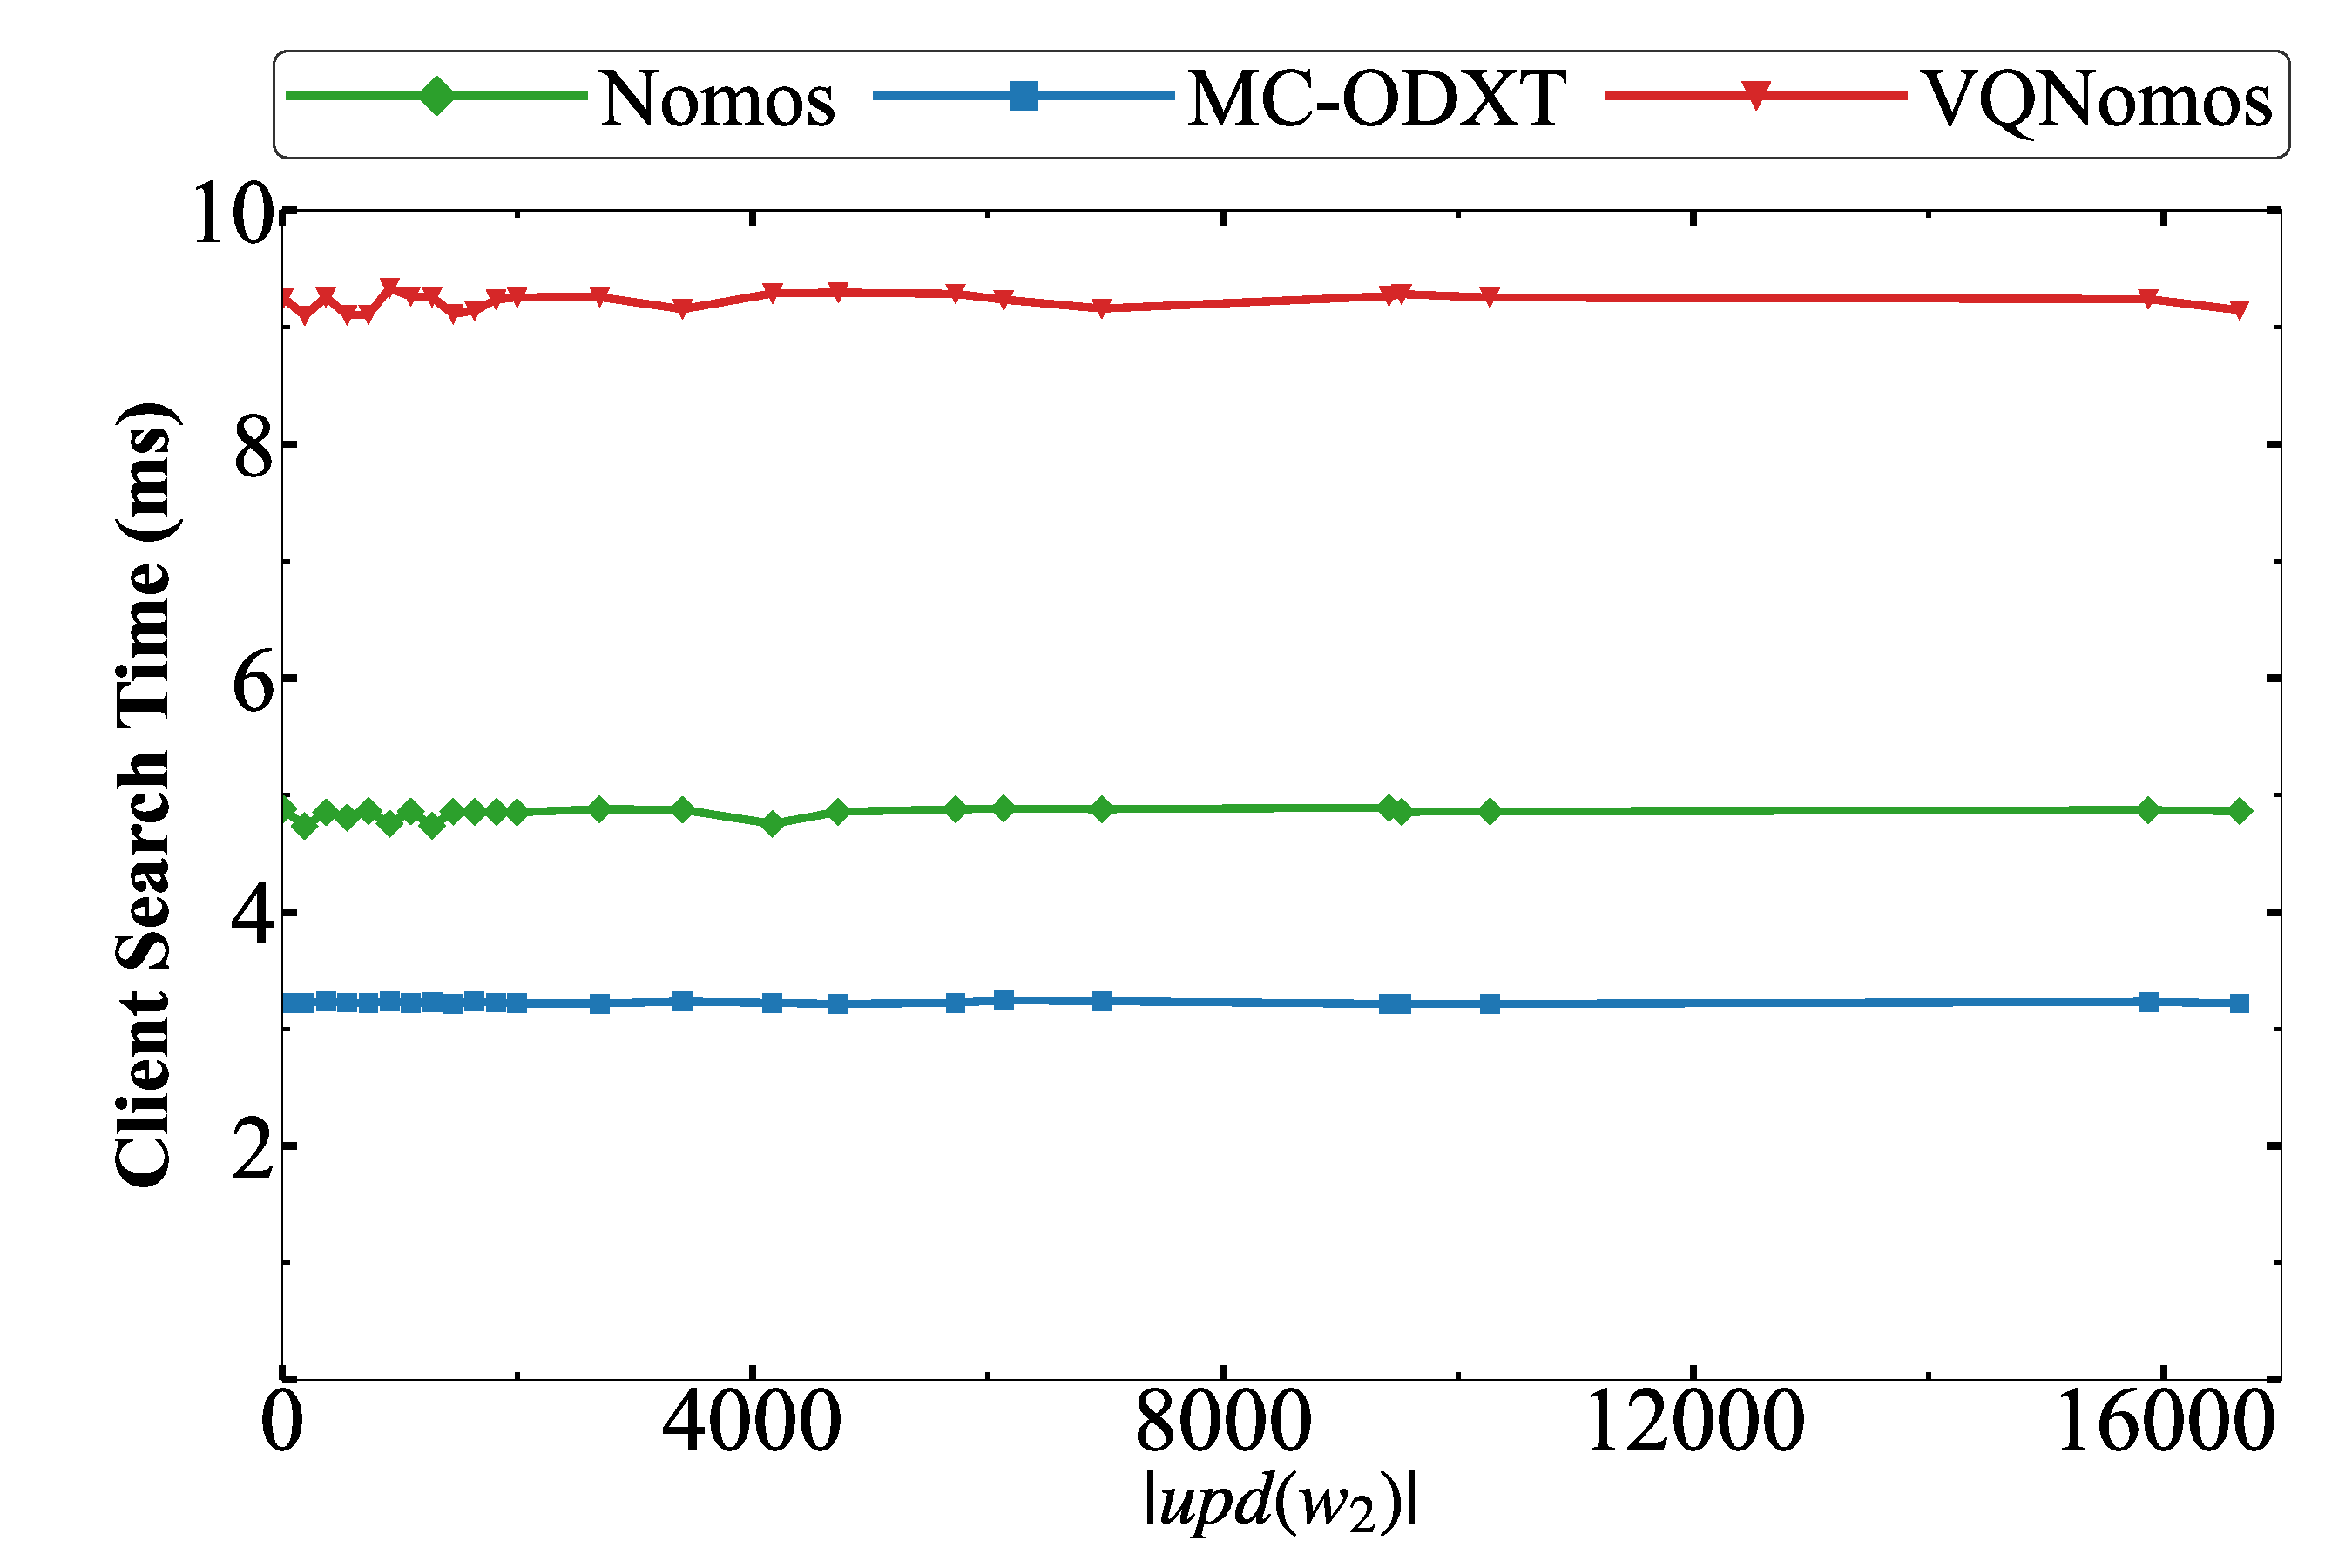
\includegraphics[width=\linewidth]
        {../figures/client_search_time_fixed_w1_figures/Crime_client_search_time_comparison.pdf}
      \caption{Crime}
    \end{subfigure}
    \hfill
    \begin{subfigure}[b]{0.32\textwidth}
      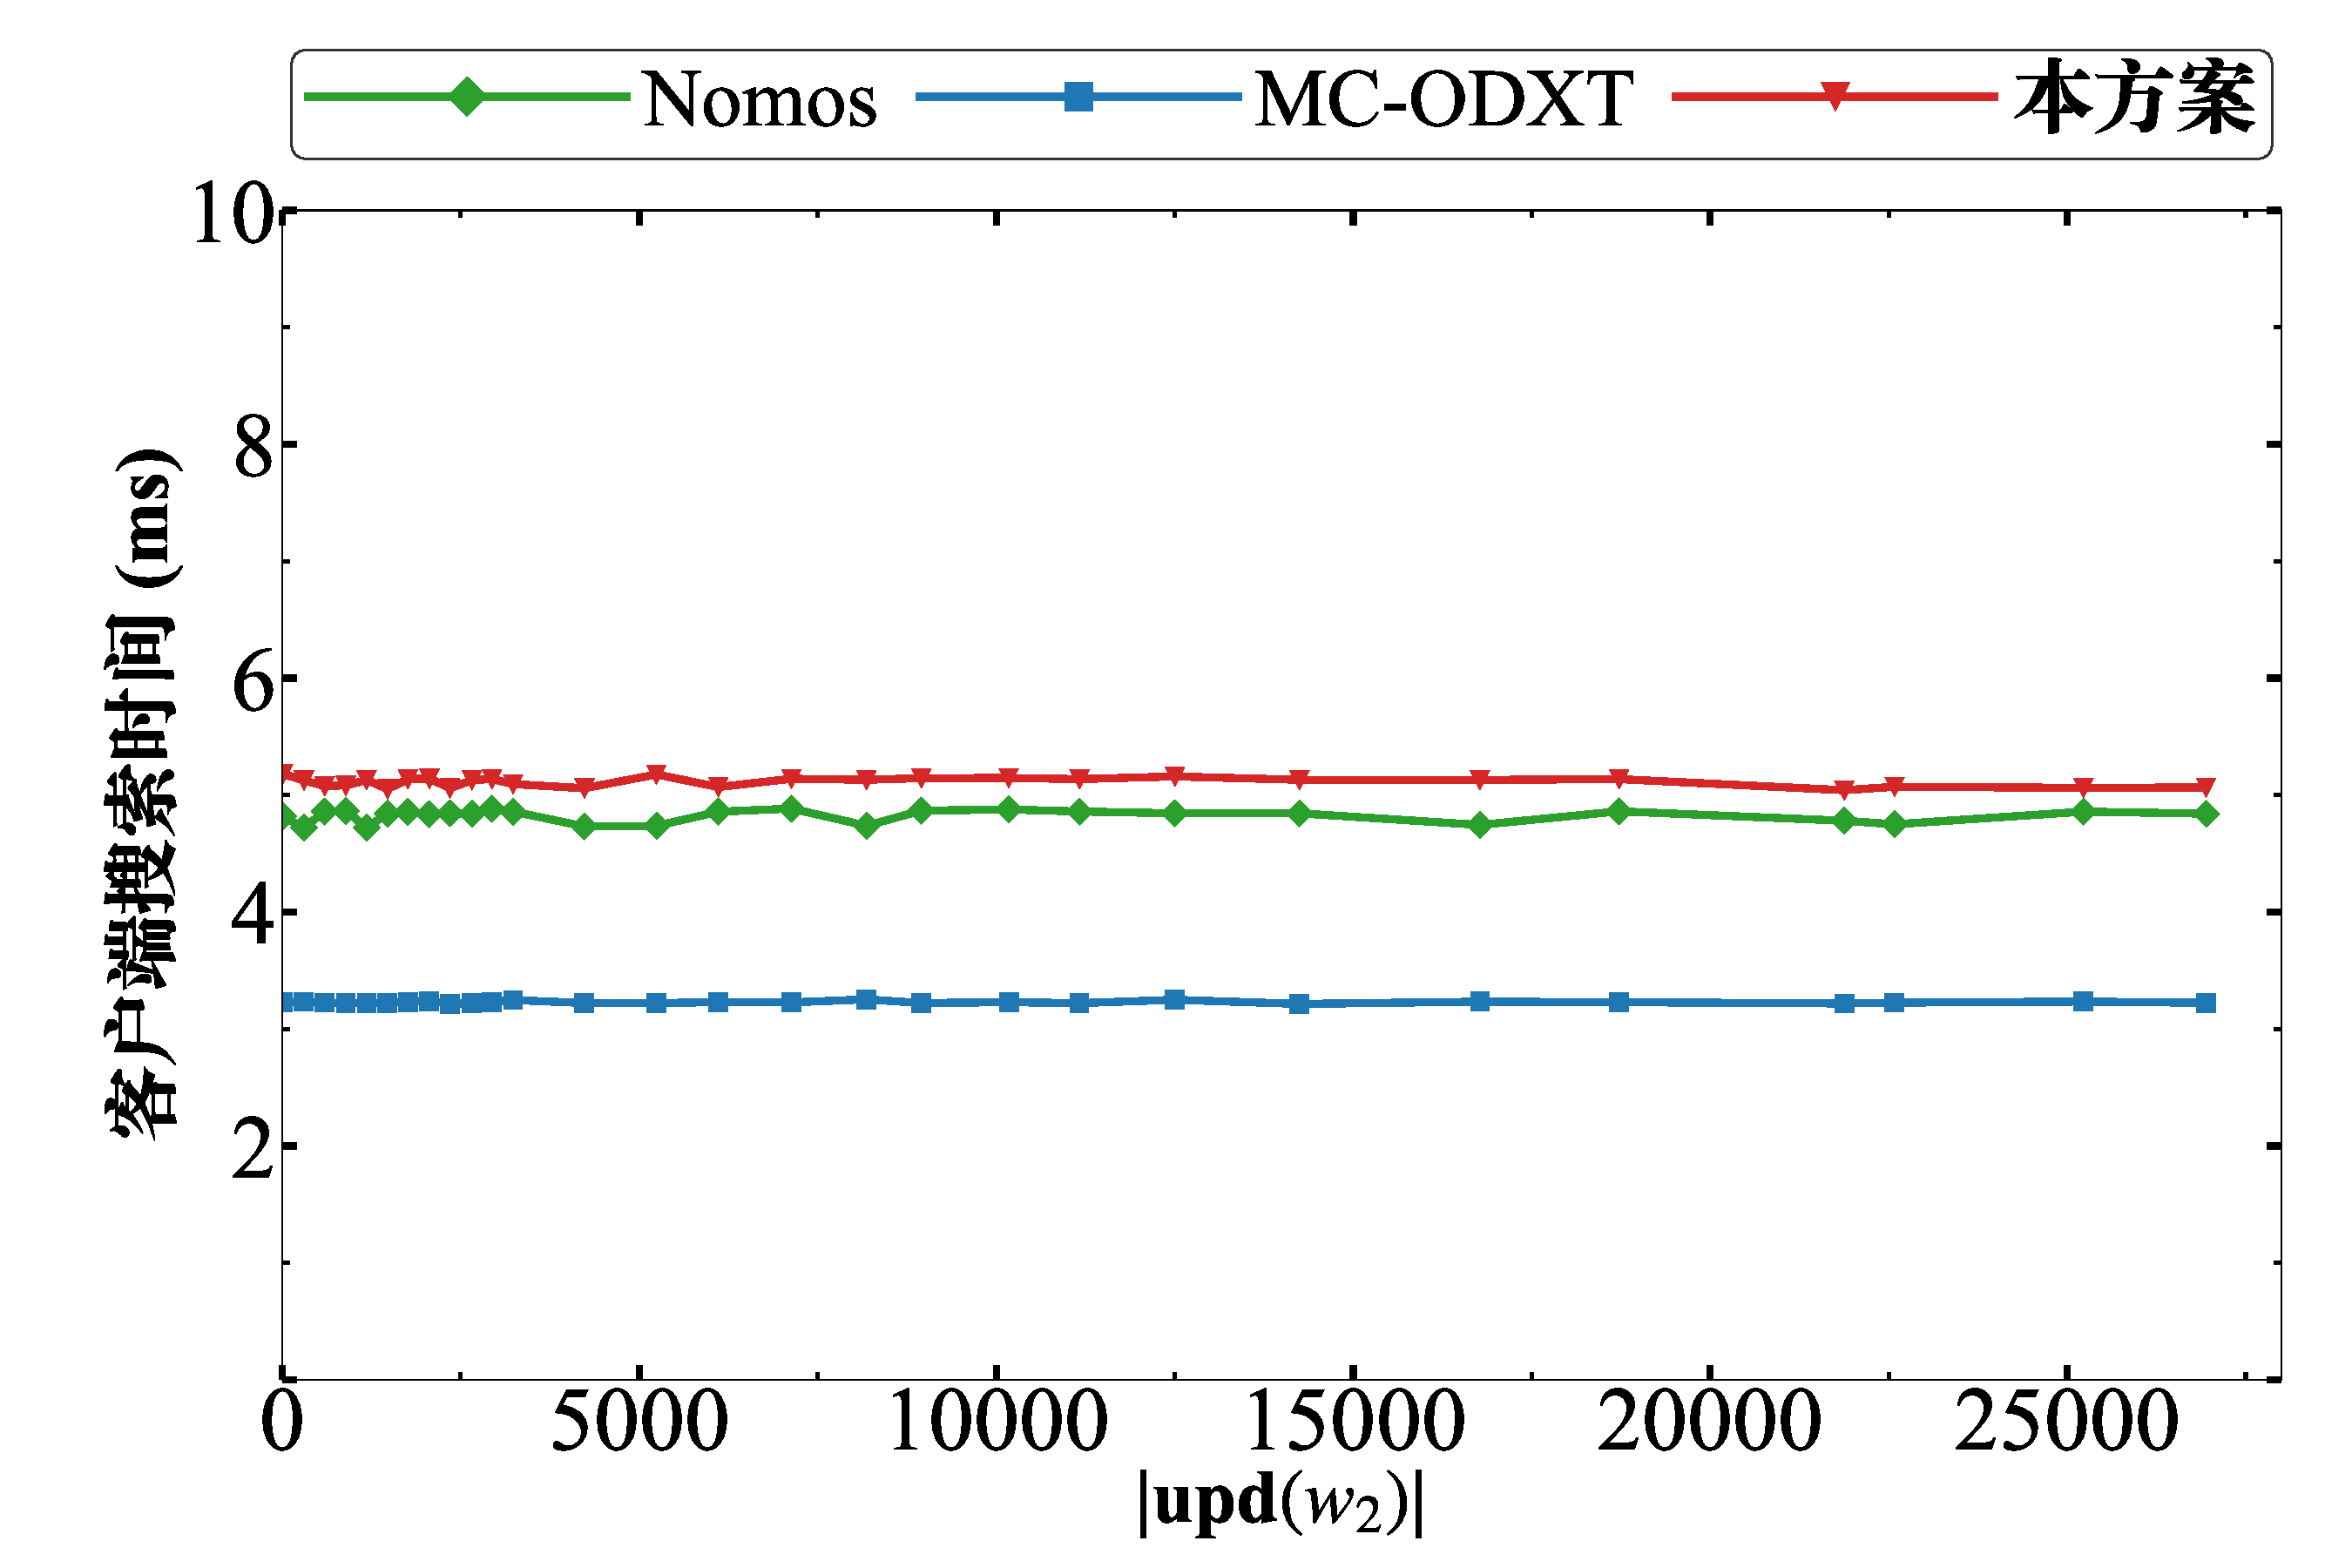
\includegraphics[width=\linewidth]
        {../figures/client_search_time_fixed_w1_figures/Enron_client_search_time_comparison.pdf}
      \caption{Enron}
    \end{subfigure}
    \hfill
    \begin{subfigure}[b]{0.32\textwidth}
      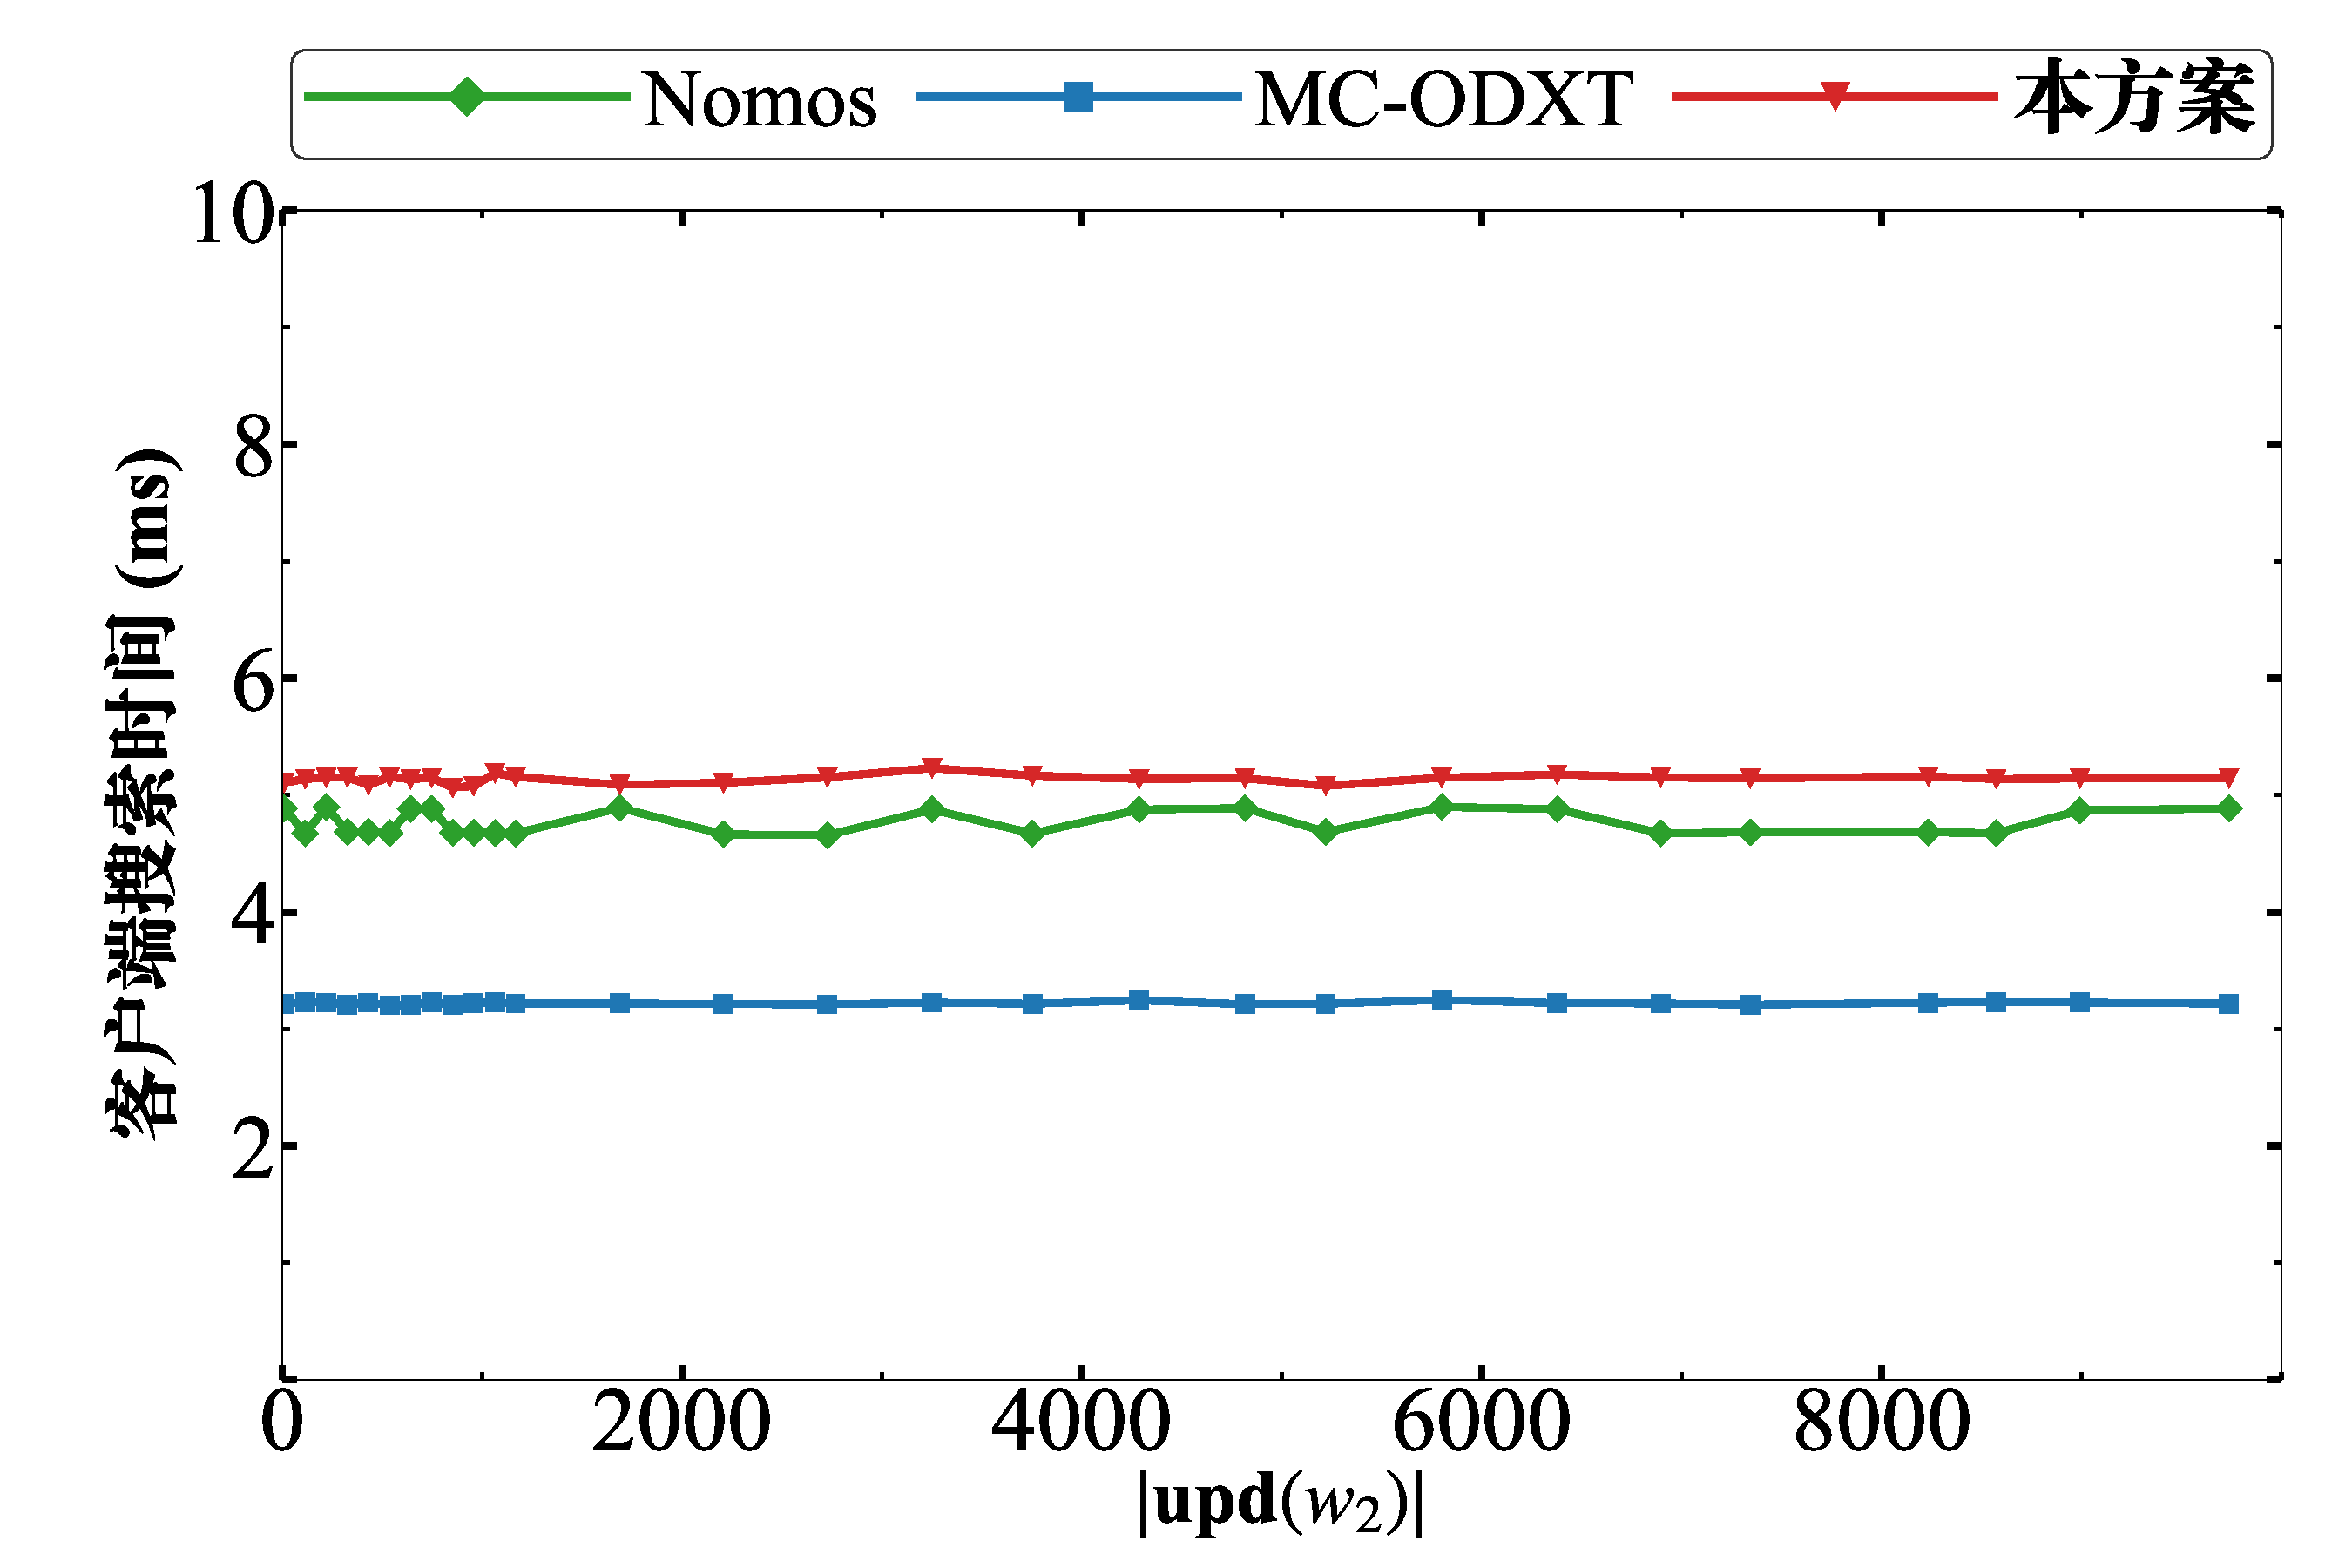
\includegraphics[width=\linewidth]
        {../figures/client_search_time_fixed_w1_figures/Wikipedia_client_search_time_comparison.pdf}
      \caption{Wiki}
    \end{subfigure}
    \caption{客户端搜索时间（与 Nomos 基线对比）}
  \end{figure}

  \begin{exampleblock}{核心结论}
    客户端搜索时间增量 $< 10\%$；
    授权管理方增量 $< 5\%$；
    搜索时间随候选集大小 $m$ 线性增长，
    符合 $O(k|Q| \cdot \mathsf{UpdateCnt}[w_s])$ 理论预测。
  \end{exampleblock}

\end{frame}

% ---- Slide: 搜索时间——服务器与管理方 ----
\begin{frame}{实验结果（二）：服务器与授权管理方搜索时间}

  \begin{columns}[T]
    \column{0.50\textwidth}
      \begin{figure}
        \begin{subfigure}[b]{0.49\textwidth}
          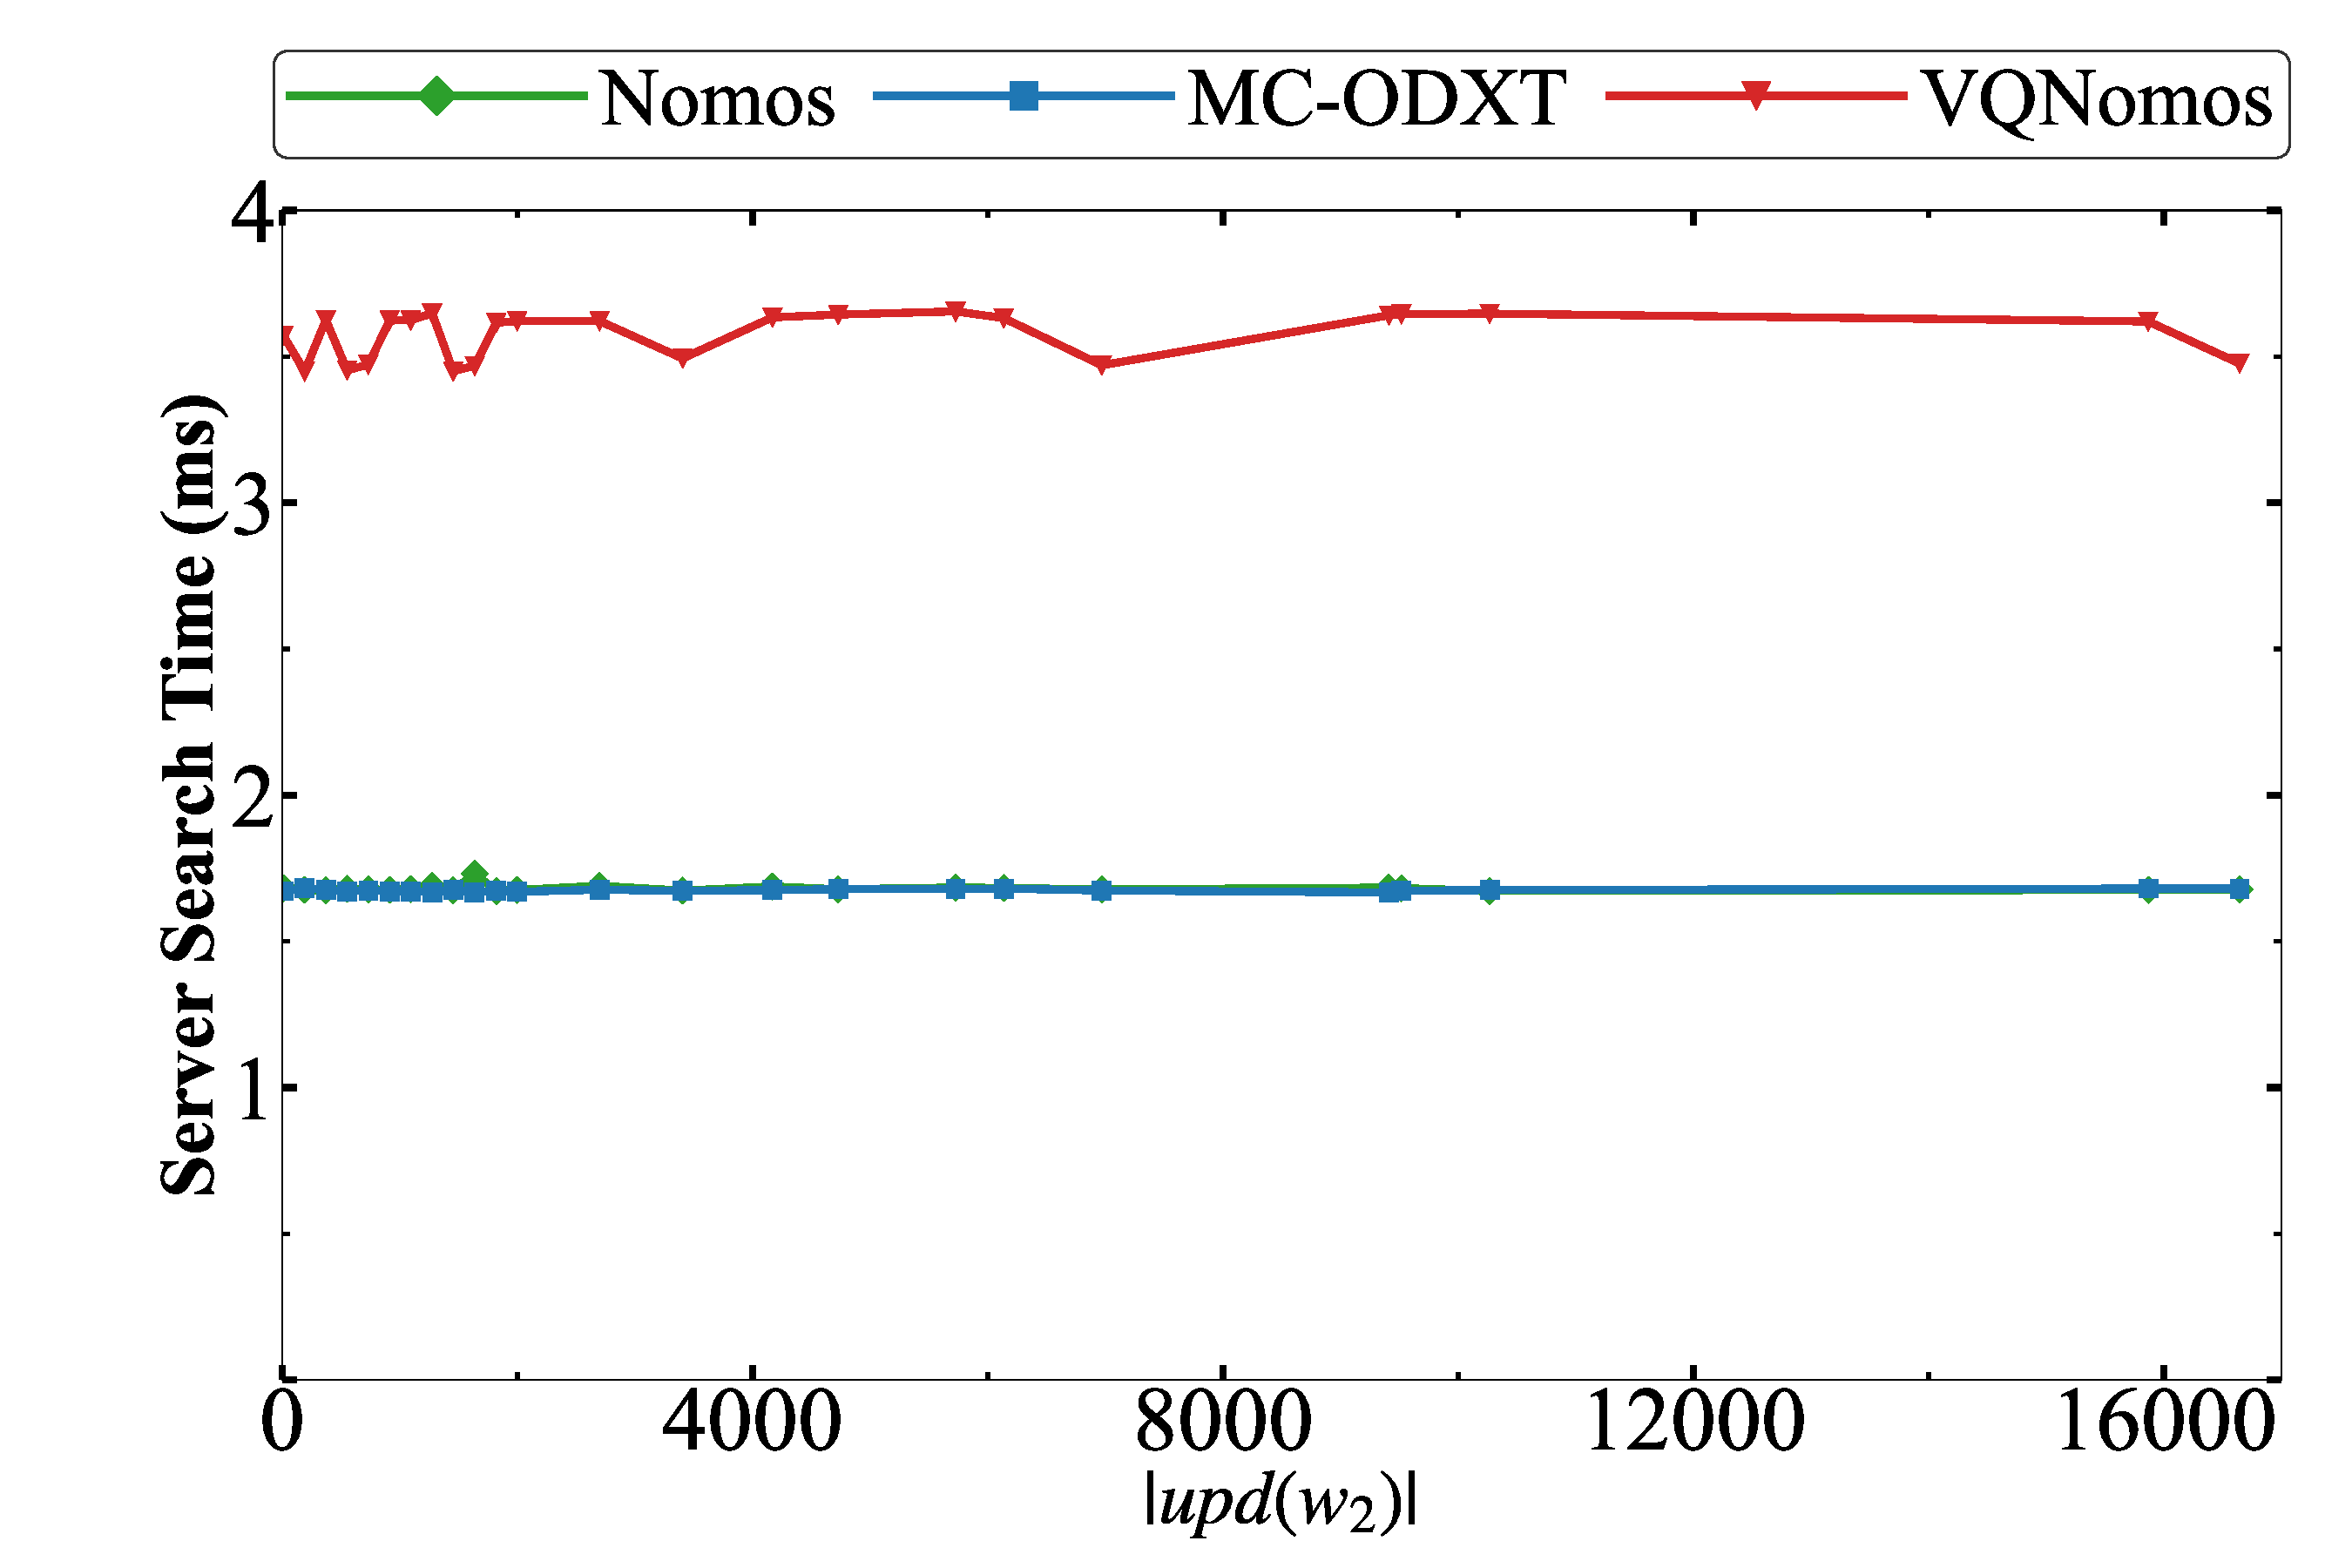
\includegraphics[width=\linewidth]
            {../figures/server_search_time_fixed_w1_figures/Crime_server_search_time_comparison.pdf}
        \end{subfigure}
        \hfill
        \begin{subfigure}[b]{0.49\textwidth}
          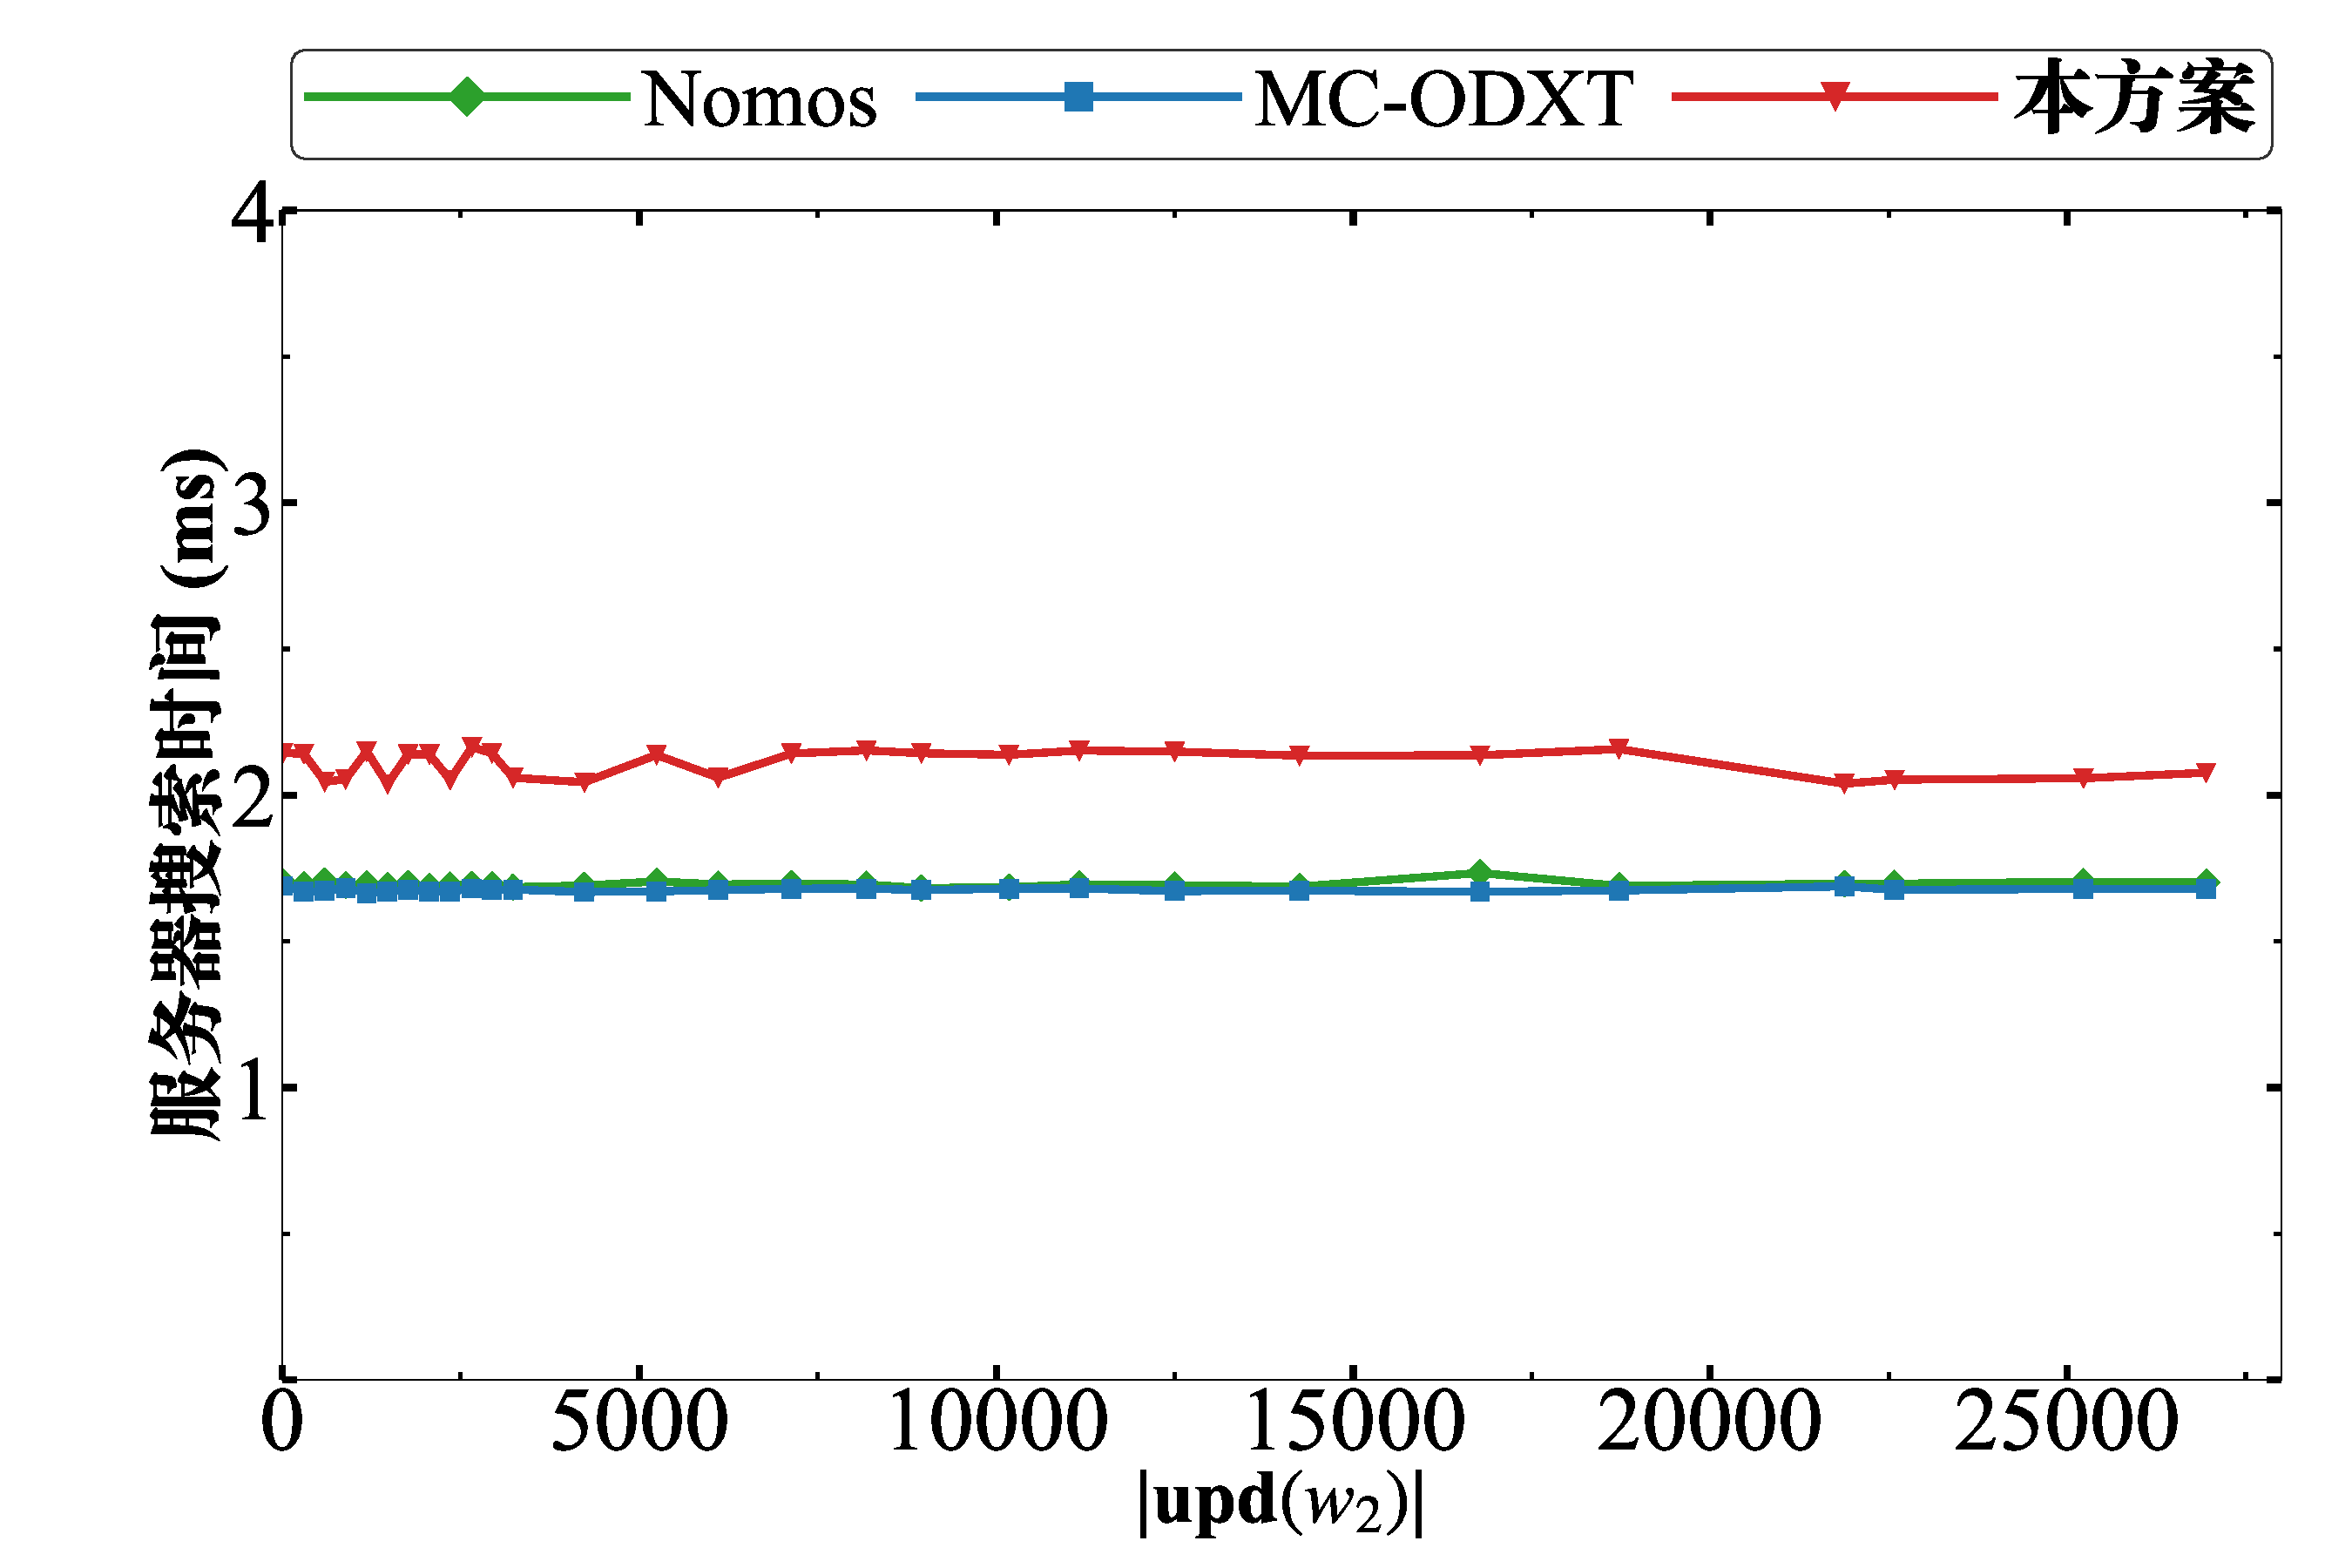
\includegraphics[width=\linewidth]
            {../figures/server_search_time_fixed_w1_figures/Enron_server_search_time_comparison.pdf}
        \end{subfigure}
        \caption{服务器搜索时间}
      \end{figure}

    \column{0.47\textwidth}
      \begin{figure}
        \begin{subfigure}[b]{0.49\textwidth}
          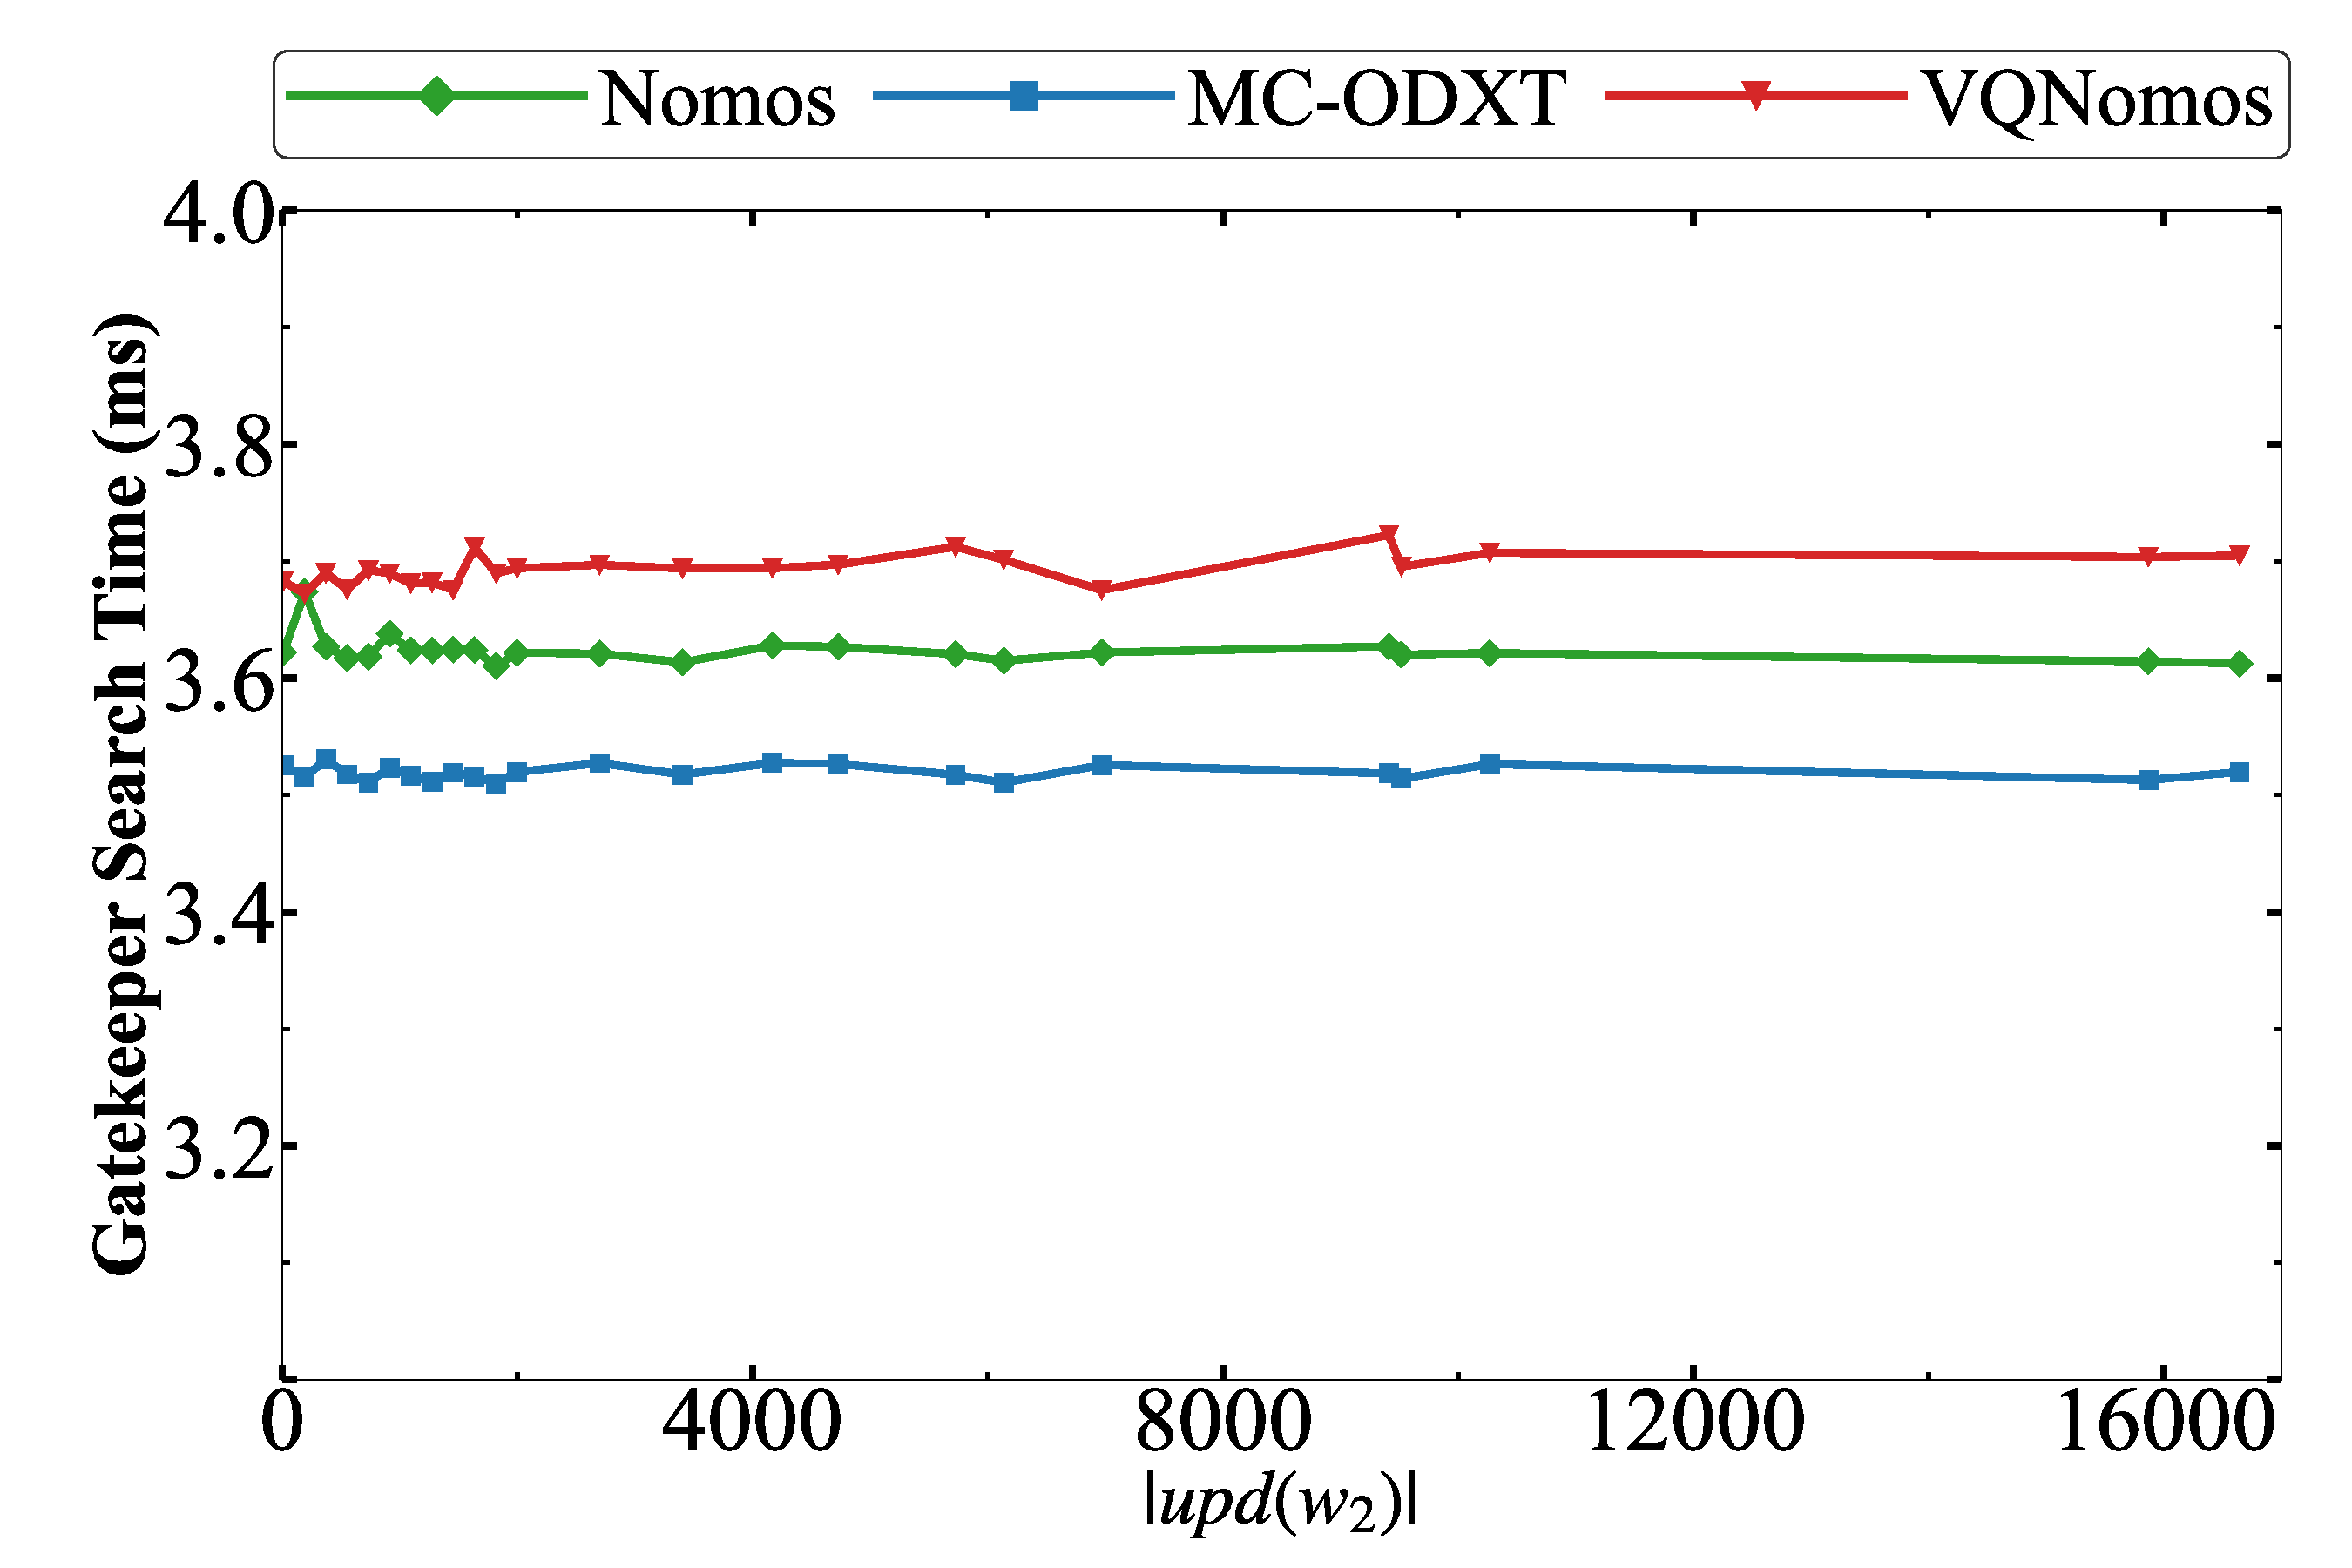
\includegraphics[width=\linewidth]
            {../figures/gatekeeper_search_time_fixed_w1_figures/Crime_gatekeeper_search_time_comparison.pdf}
        \end{subfigure}
        \hfill
        \begin{subfigure}[b]{0.49\textwidth}
          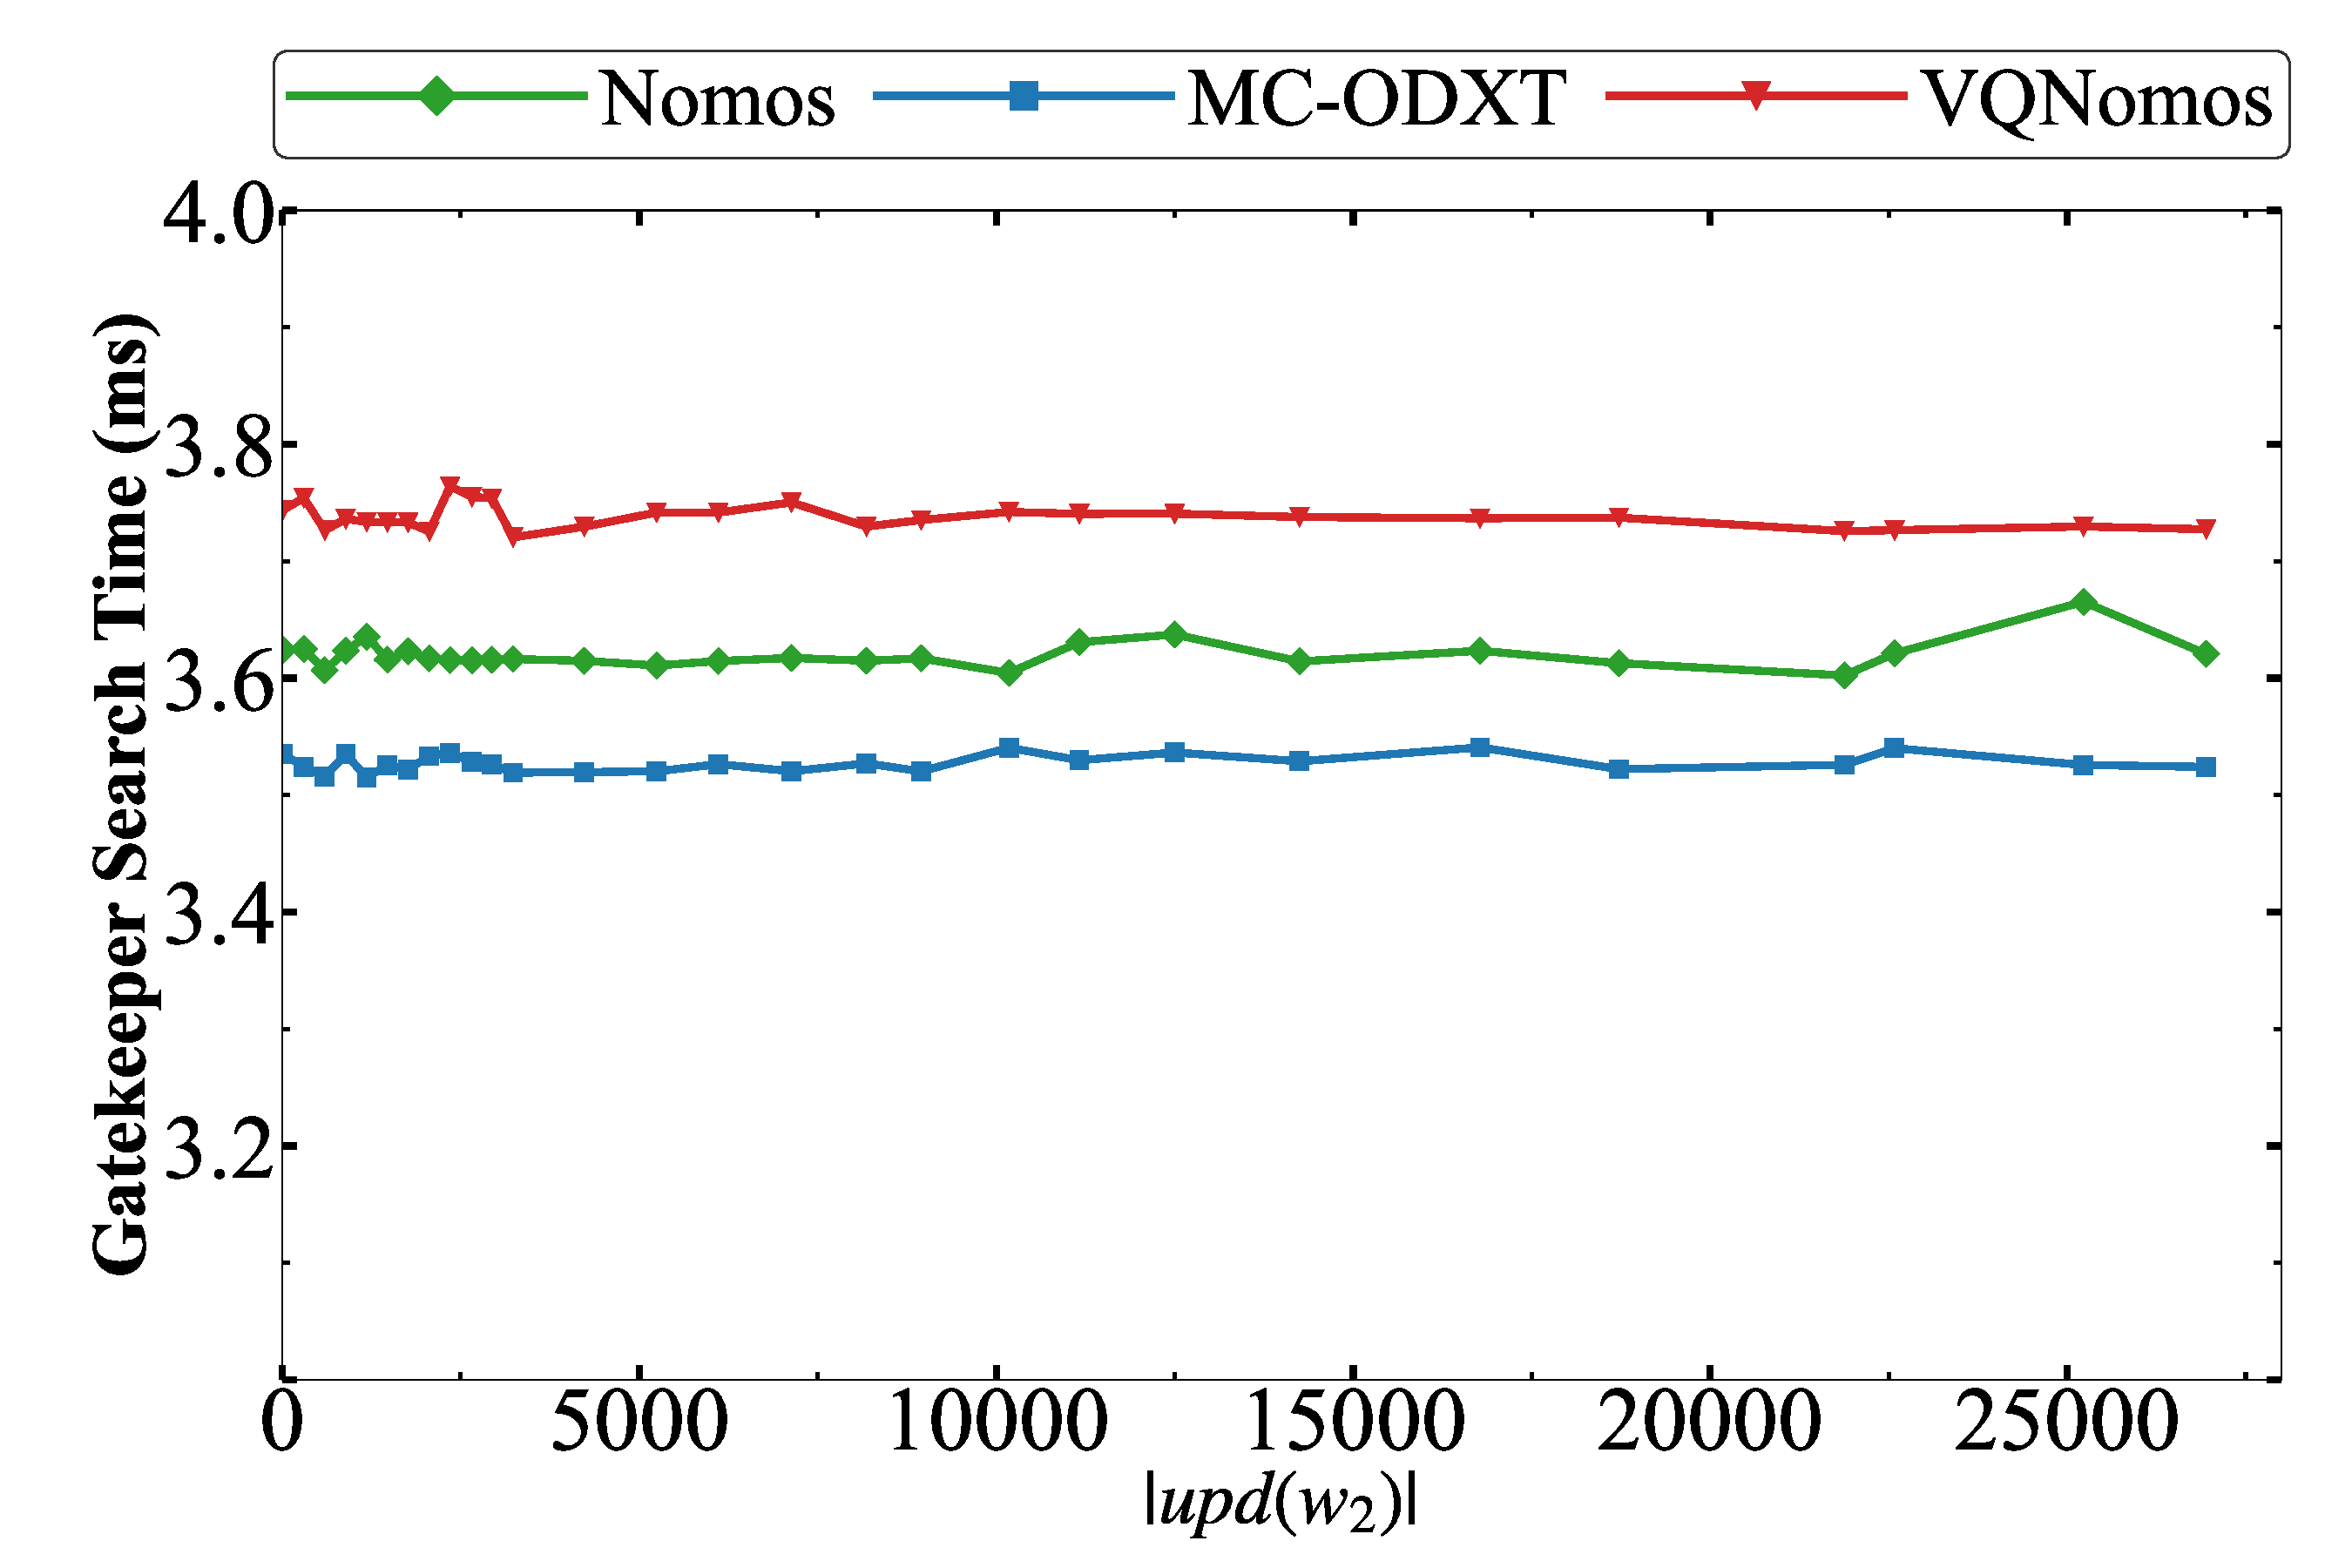
\includegraphics[width=\linewidth]
            {../figures/gatekeeper_search_time_fixed_w1_figures/Enron_gatekeeper_search_time_comparison.pdf}
        \end{subfigure}
        \caption{授权管理方搜索时间}
      \end{figure}
  \end{columns}

  \begin{exampleblock}{服务器时间增量 $< 20\%$，理论与实验高度吻合}
  \end{exampleblock}

\end{frame}

% ---- Slide: 存储开销 ----
\begin{frame}{实验结果（三）：存储开销}

  \begin{columns}[T]
    \column{0.56\textwidth}
      \begin{figure}
        \begin{subfigure}[b]{0.48\textwidth}
          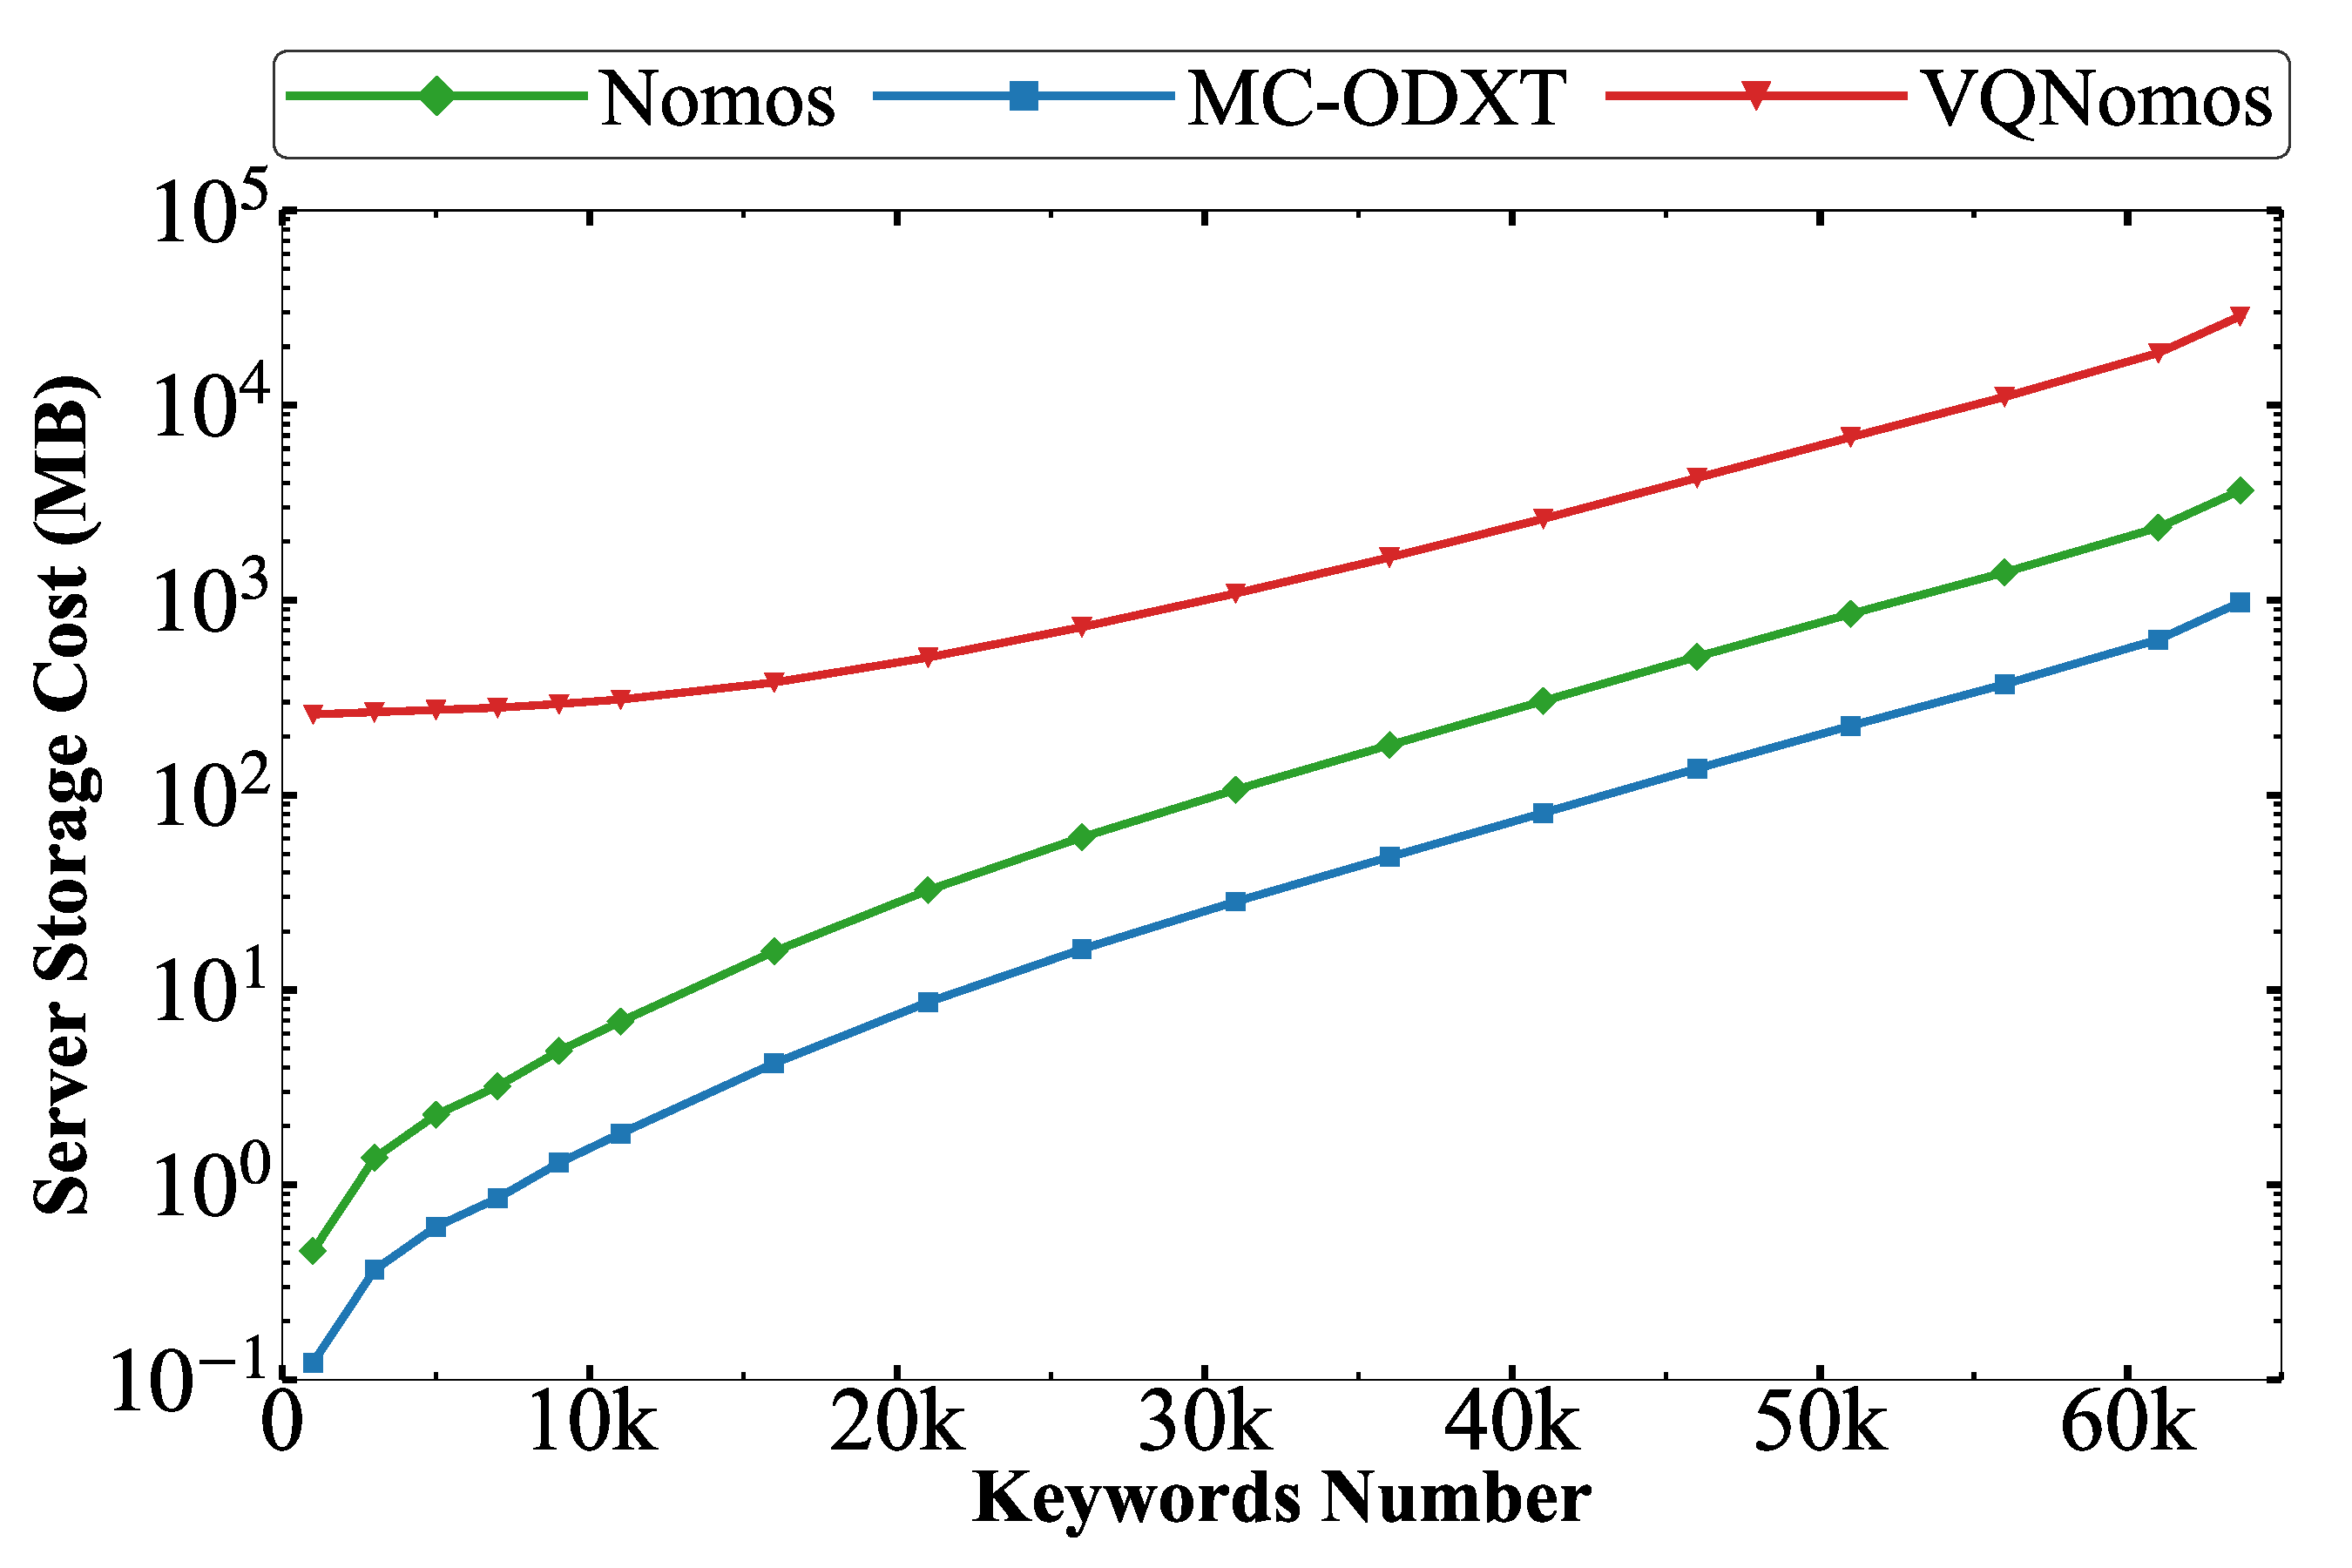
\includegraphics[width=\linewidth]
            {../figures/nomos_server_storage/Crime_server_storage_comparison.pdf}
          \caption{Crime}
        \end{subfigure}
        \hfill
        \begin{subfigure}[b]{0.48\textwidth}
          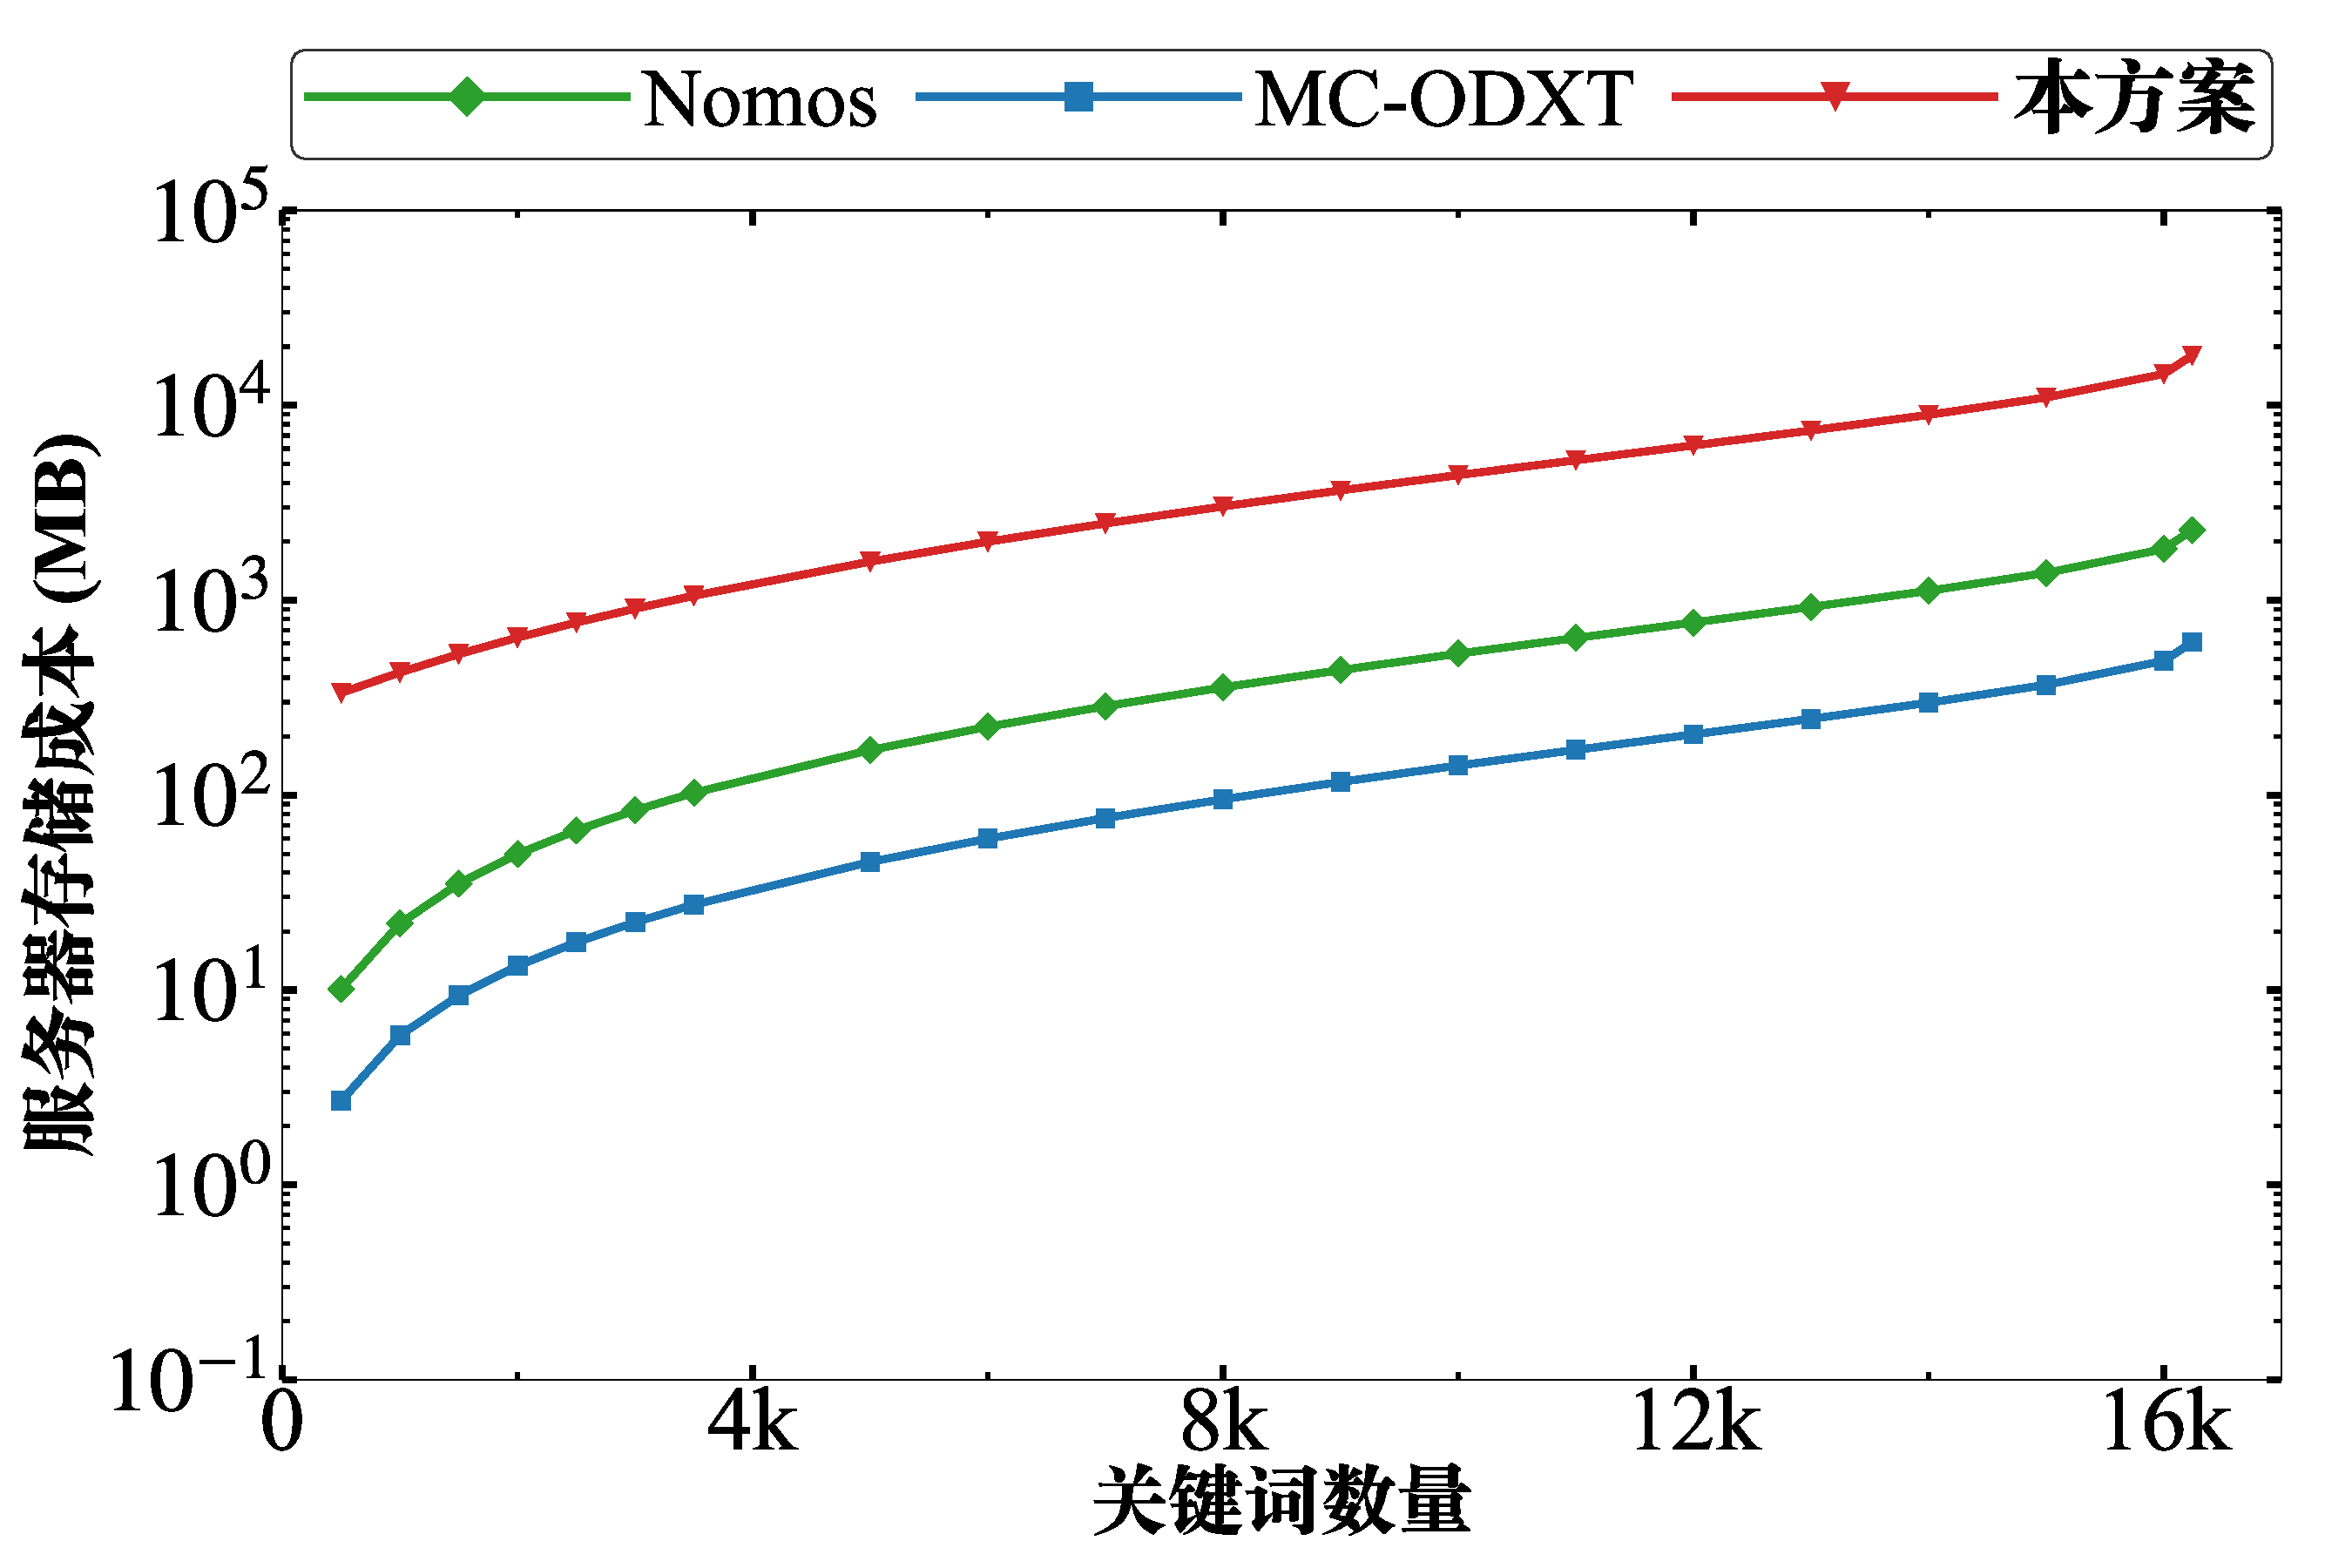
\includegraphics[width=\linewidth]
            {../figures/nomos_server_storage/Enron_server_storage_comparison.pdf}
          \caption{Enron}
        \end{subfigure}
        \caption{服务器存储开销（相对 Nomos 对比）}
      \end{figure}

    \column{0.41\textwidth}
      \begin{block}{存储汇总}
        \small
        \begin{tabular}{lll}
          \toprule
          \textbf{数据集} & \textbf{Nomos} & \textbf{本文} \\
          \midrule
          Crime & 765\,MB & 7.4\,GB \\
          Enron & 497\,MB & 4.8\,GB \\
          Wiki  & 437\,MB & 4.2\,GB \\
          \bottomrule
        \end{tabular}
      \end{block}

      \vspace{0.4em}
      \begin{exampleblock}{分析}
        \small
        \begin{itemize}
          \item 服务器存储膨胀源于 MPos $+$ MTree 结构
          \item 渐近 $O(N\ell\lambda)$，可通过压缩优化
          \item \textbf{客户端存储增量 $< 0.1\%$}，对用户透明
        \end{itemize}
      \end{exampleblock}
  \end{columns}

\end{frame}

% ---- Slide: 通信开销 ----
\begin{frame}{实验结果（四）：通信开销}

  \begin{columns}[T]
    \column{0.56\textwidth}
      \begin{figure}
        \begin{subfigure}[b]{0.48\textwidth}
          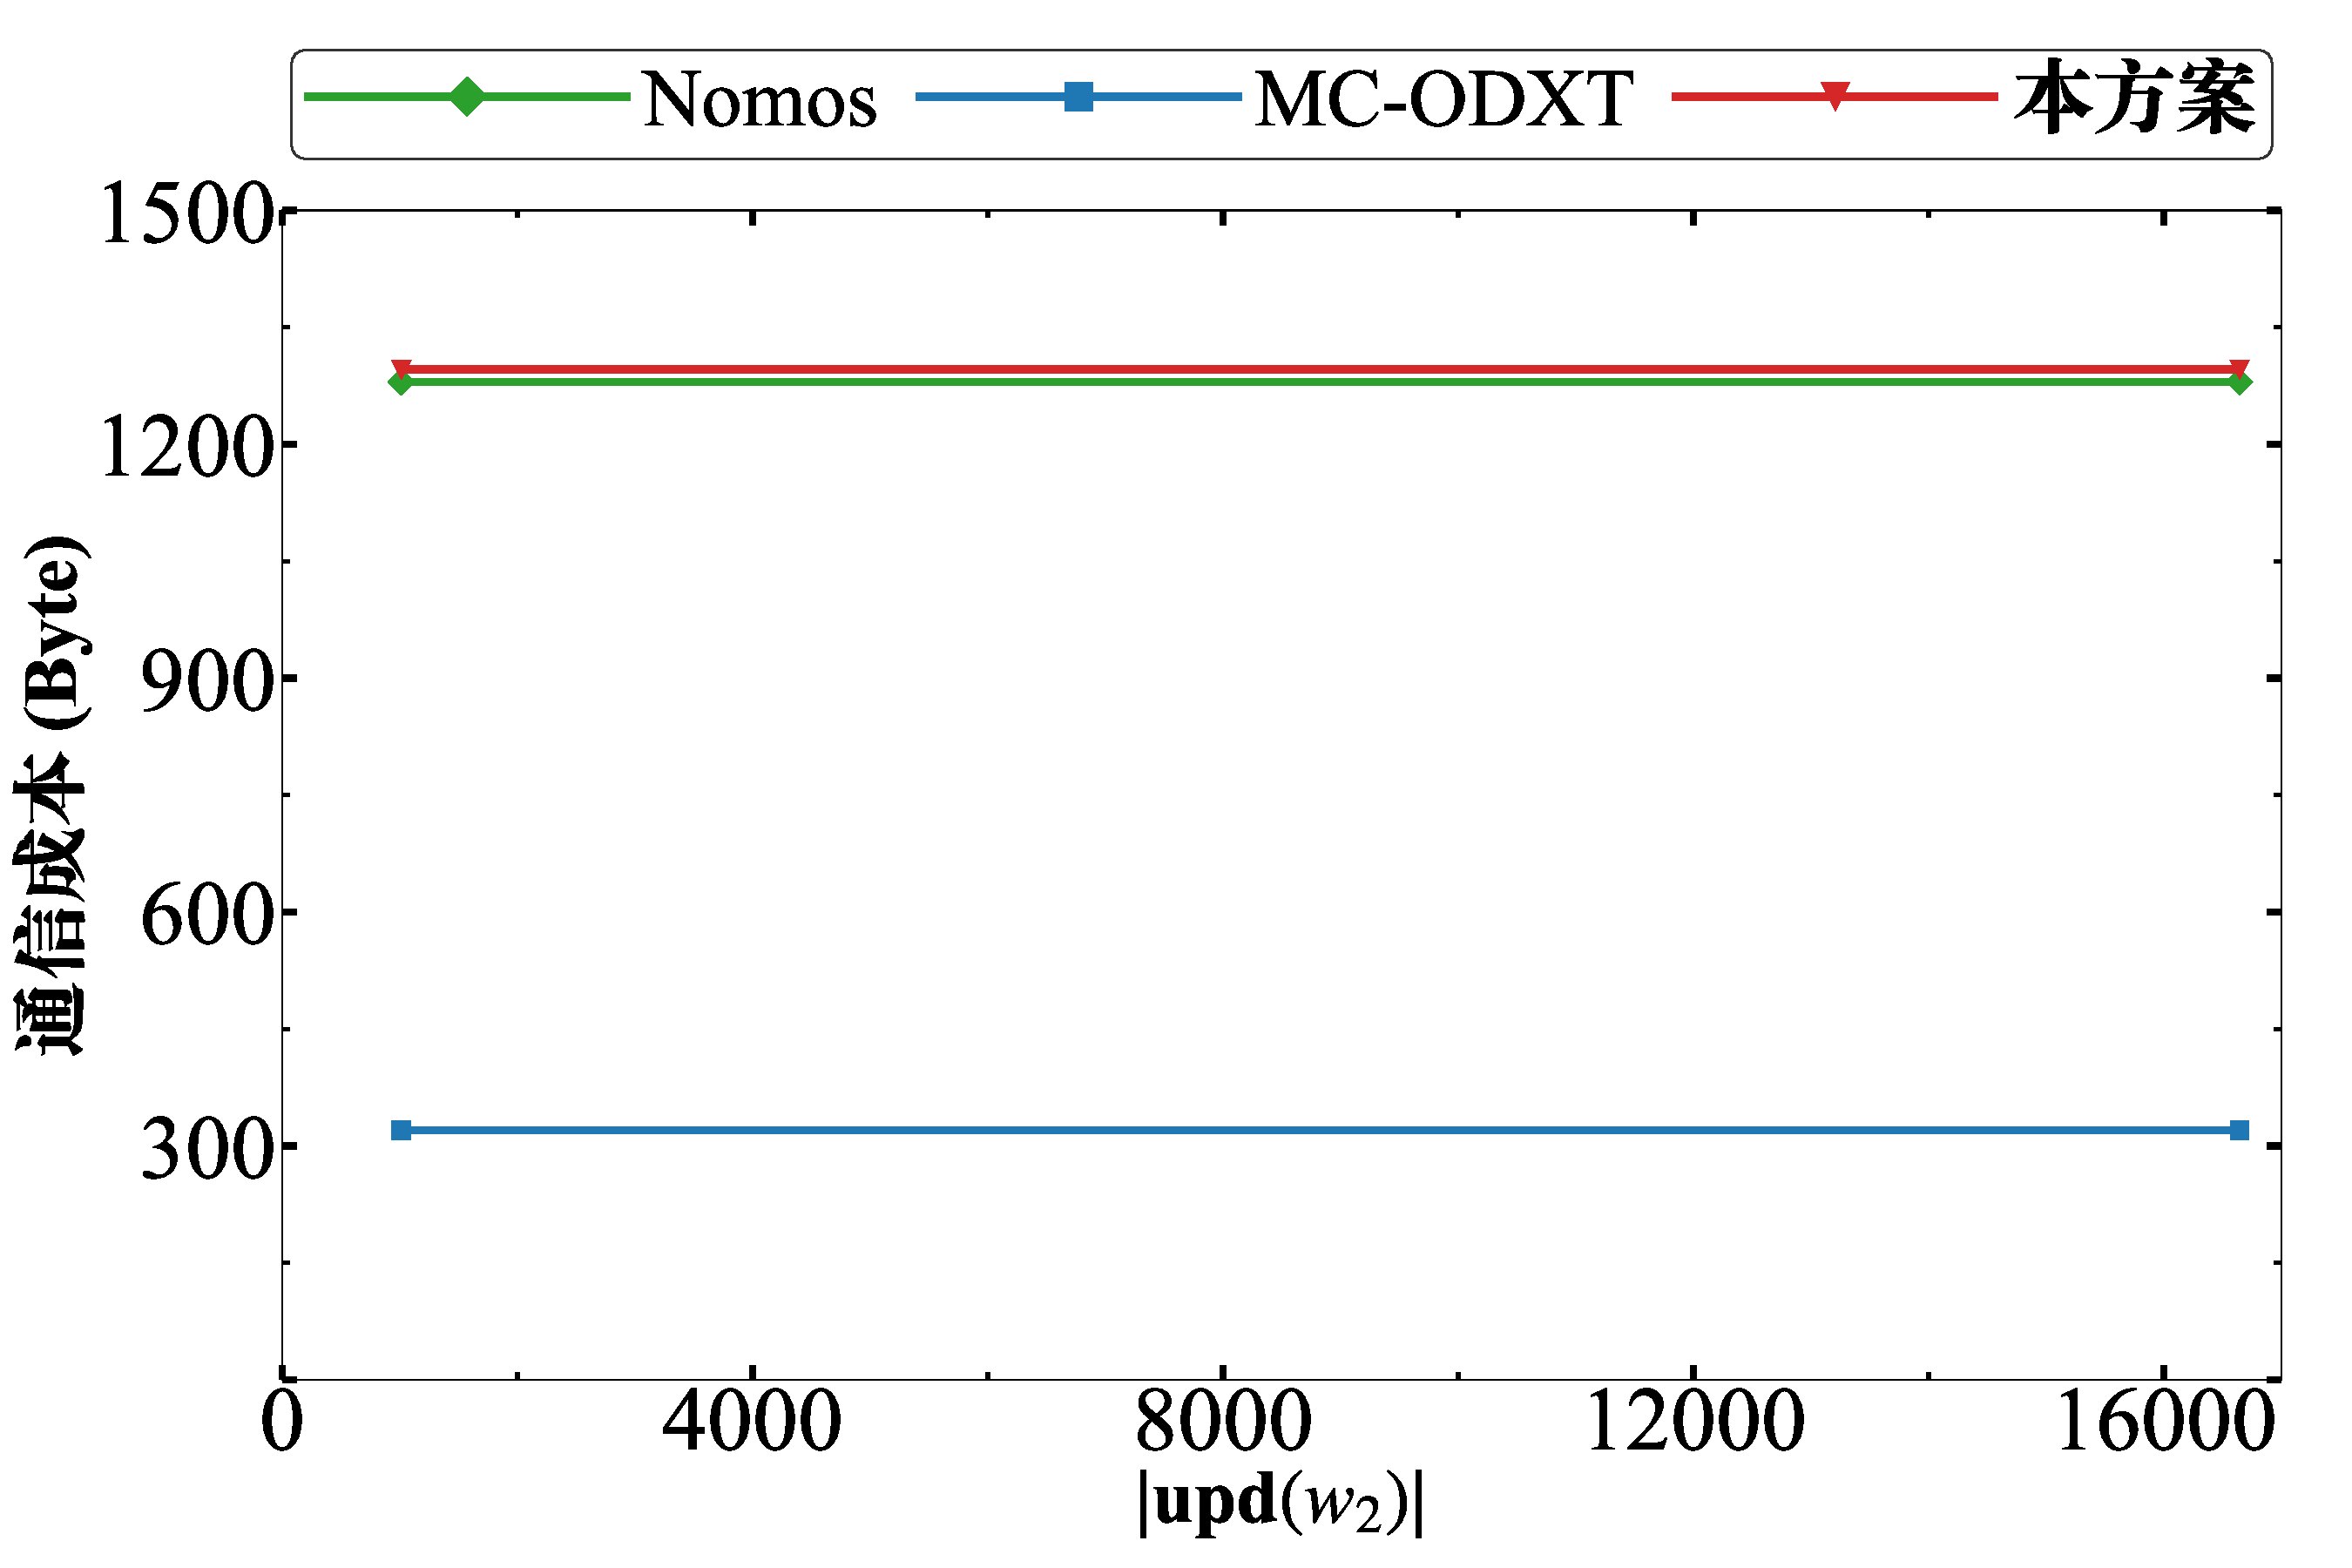
\includegraphics[width=\linewidth]
            {../figures/nomos_client_communication_w1/Crime_client_communication_comparison.pdf}
          \caption{Crime}
        \end{subfigure}
        \hfill
        \begin{subfigure}[b]{0.48\textwidth}
          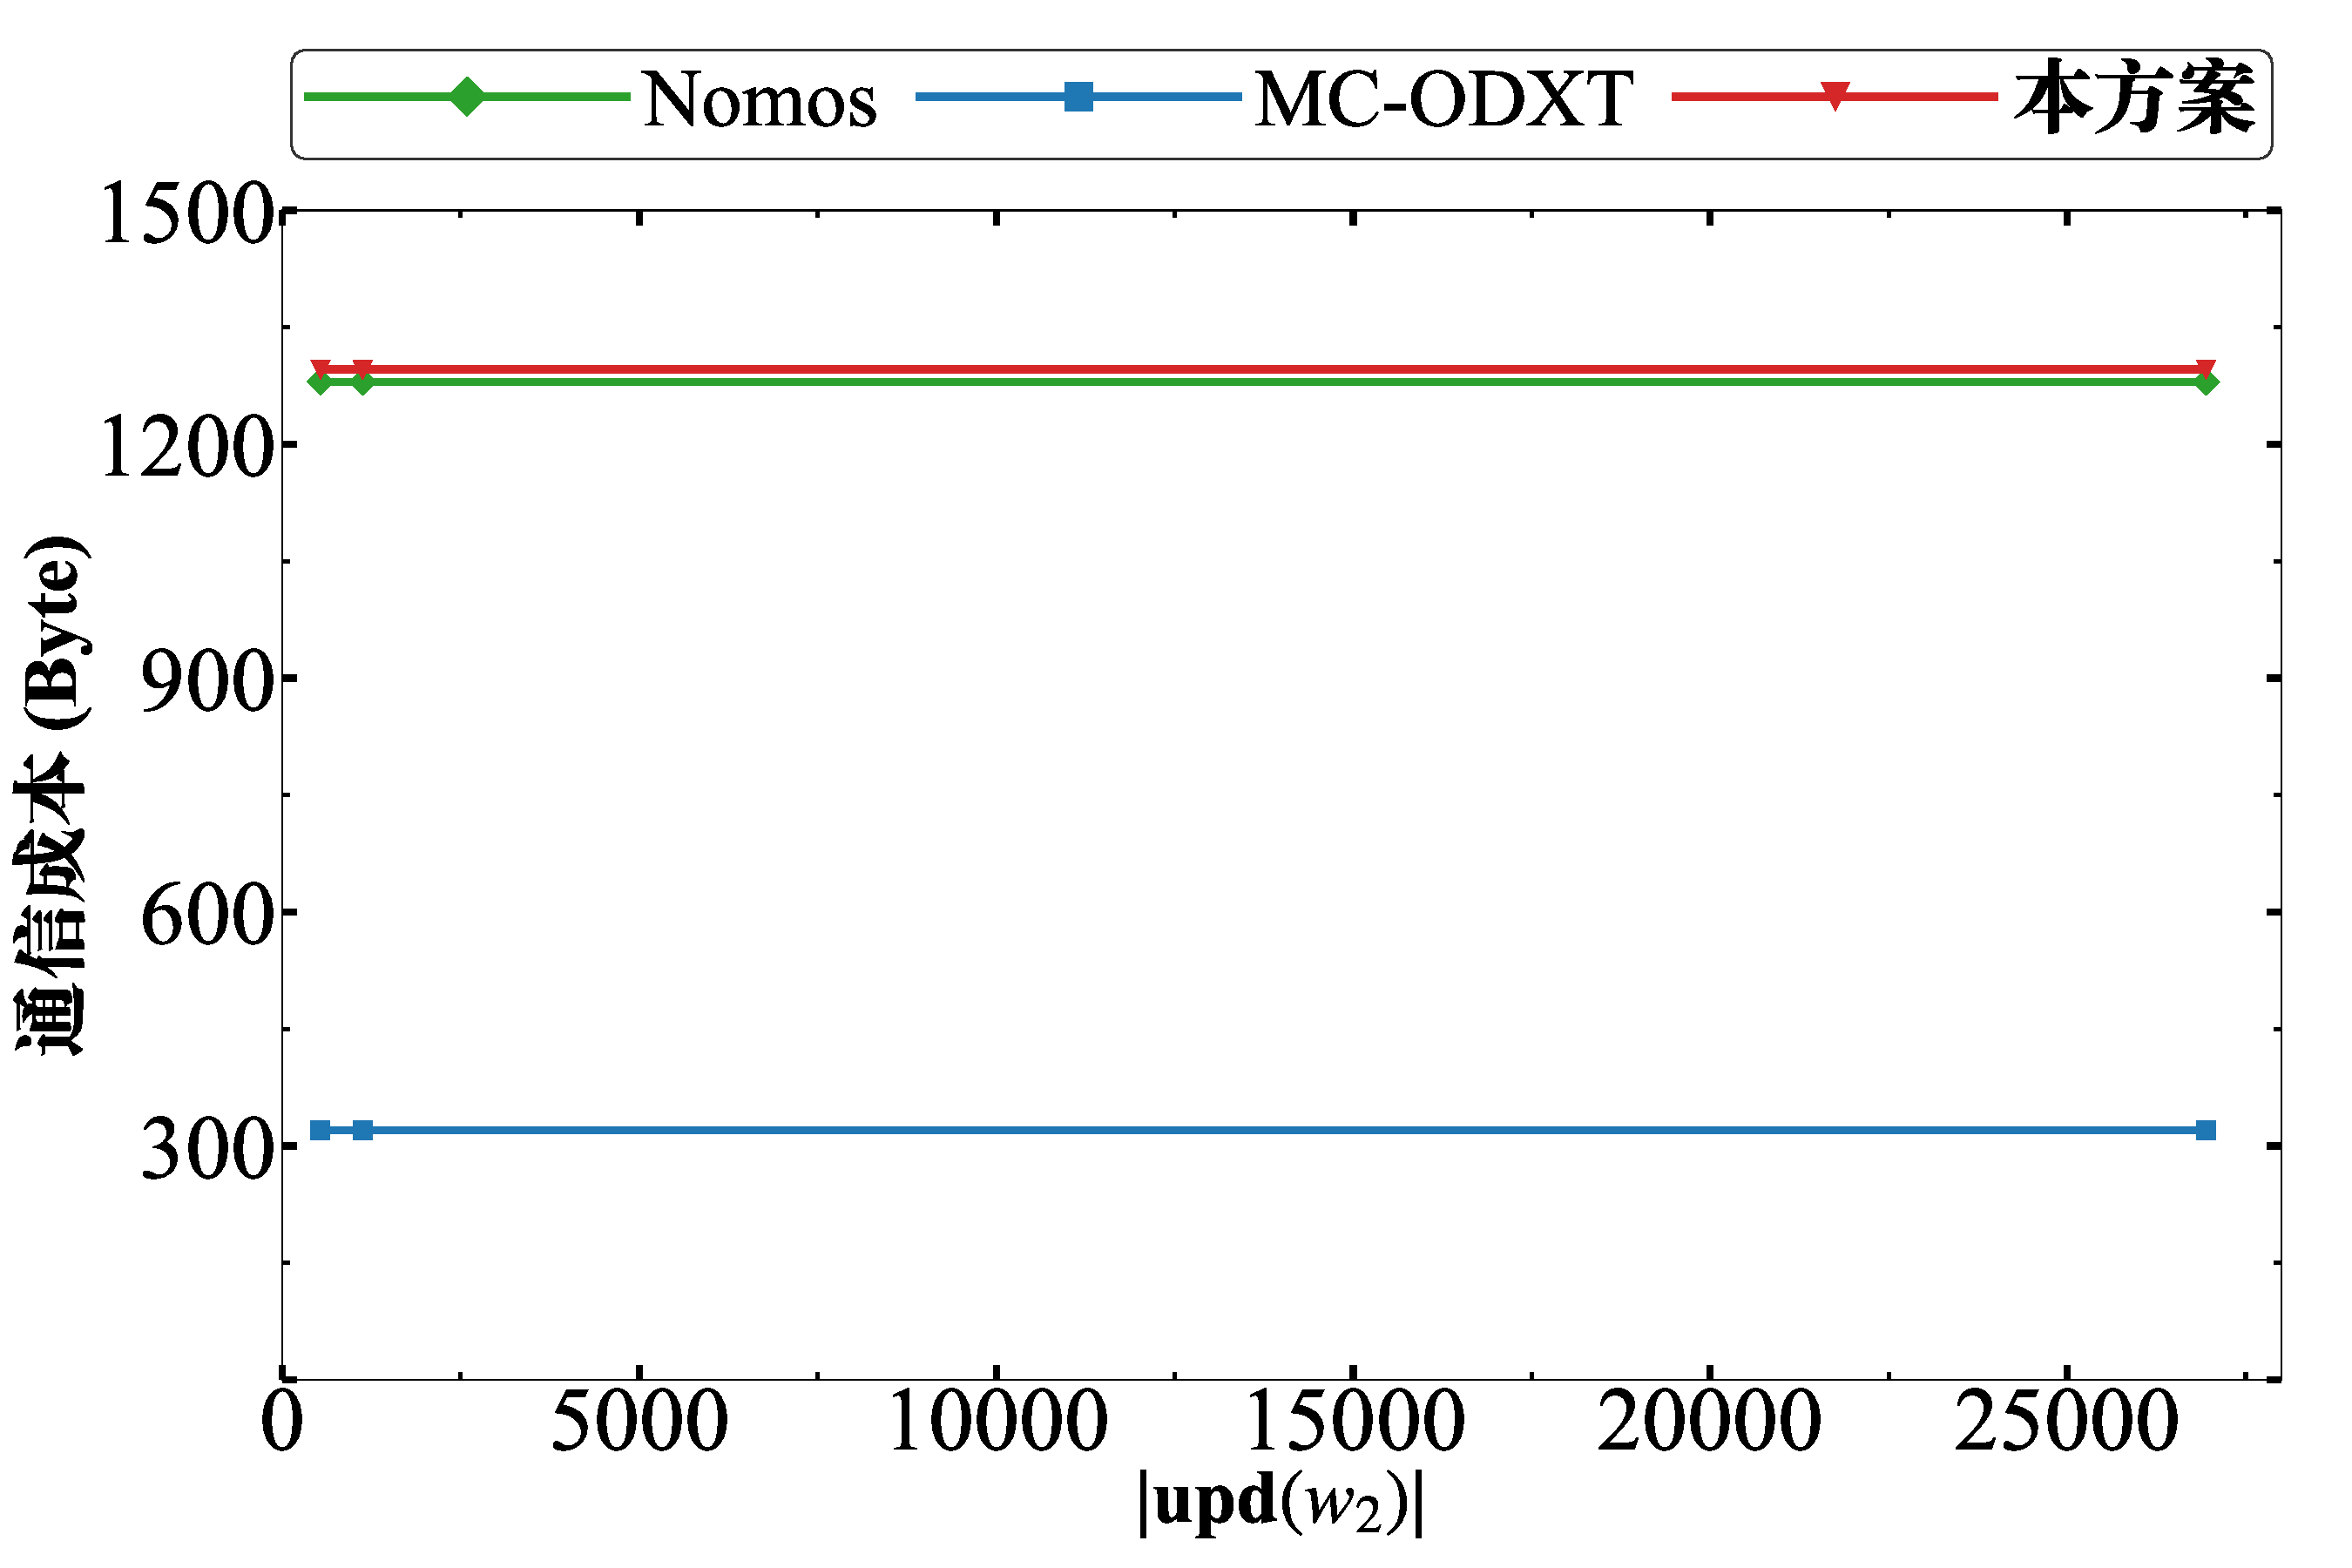
\includegraphics[width=\linewidth]
            {../figures/nomos_client_communication_w1/Enron_client_communication_comparison.pdf}
          \caption{Enron}
        \end{subfigure}
        \caption{客户端通信开销（相对 Nomos 对比）}
      \end{figure}

    \column{0.41\textwidth}
      \begin{block}{通信开销分析}
        \small
        \begin{itemize}
          \item \textbf{客户端上传增量}：$< 0.2\%$\\
                （仅版本号 8\,B + 采样索引 8\,B）
          \item \textbf{服务器下发增量}：\\
                $O(k(\log M + \log \ell))$ 哈希值
          \item 选择性开封将单条关系通信\\
                从 $O(\ell|\mathbb{G}|)$ 降至 $O(k(|\mathbb{G}|+\lambda\log\ell))$
        \end{itemize}
      \end{block}

      \vspace{0.3em}
      \begin{exampleblock}{综合结论}
        \small
        客户端与通信侧开销几乎可忽略，
        服务器侧存储为主要代价，
        整体轻量，适合多用户云端部署。
      \end{exampleblock}
  \end{columns}

\end{frame}

% ============================================================
%  第七章：总结与展望
% ============================================================
\section{总结与展望}

% ---- Slide: 主要贡献 ----
\begin{frame}{总结与主要贡献}

  \begin{block}{贡献一：可验证资格检验机制 $\pi_\mathsf{VQ}$}
    \begin{itemize}
      \item 在 RBF 基础上引入 Merkle Hash Tree 承诺层与版本锚定签名
      \item 将布尔判定升级为可独立验证的密码学证明（支持双向证据）
      \item 形式化证明：绑定健全性、版本一致性、条件完整性
    \end{itemize}
  \end{block}

  \begin{block}{贡献二：基于 Merkle-Open 的地址绑定验证}
    \begin{itemize}
      \item 在 OPRF 盲化下保护查询隐私的前提下验证地址归属
      \item 单条关系搜索通信从 $O(\ell|\mathbb{G}|)$ 降至 $O(k(|\mathbb{G}|+\lambda\log\ell))$
      \item 形式化证明地址绑定健全性（含 ExistTree 存在性承诺）
    \end{itemize}
  \end{block}

  \begin{block}{贡献三：组合可验证性与实验验证}
    \begin{itemize}
      \item 两层机制建立从地址归属正确性到位值真实性的完整验证链路
      \item 在 Crime/Enron/Wiki 三个数据集上客户端开销增量 $< 10\%$
      \item 理论分析与实验结果高度吻合，证实机制在实际部署中的可行性
    \end{itemize}
  \end{block}

\end{frame}

% ---- Slide: 局限与未来工作 ----
\begin{frame}{局限与未来研究方向}

  \begin{columns}[T]
    \column{0.48\textwidth}
      \begin{alertblock}{现有工作的局限}
        \begin{itemize}
          \item 依赖服务器如实返回目标候选条目，
                未涵盖 TSet 链式索引的\textbf{枚举完整性}验证
          \item 服务器侧存储开销相对基线有显著增长
          \item 仅覆盖合取查询语义，未扩展至析取与布尔组合
        \end{itemize}
      \end{alertblock}

    \column{0.48\textwidth}
      \begin{exampleblock}{未来研究方向}
        \begin{itemize}
          \item[1.] \textbf{TSet 枚举完整性}：\\
                对链式结构引入 Merkle 承诺，
                验证候选链长与起始地址
          \item[2.] \textbf{扩展查询语义}：\\
                研究 Merkle-Open 在析取与布尔组合查询下的扩展
          \item[3.] \textbf{泄露与开销建模}：\\
                评估语义扩展对泄露函数与通信量的影响，
                指导存储裁剪优化
        \end{itemize}
      \end{exampleblock}
  \end{columns}

\end{frame}

% ---- Slide: 致谢 ----
\begin{frame}{致\quad 谢}

  \begin{center}
    \vspace{0.5em}
    {\large 衷心感谢\\[0.5em]}
    {\large 导师 XXX 教授多年来在学术研究上的悉心指导\\[0.4em]}
    {\large 感谢各位师兄师姐师弟师妹的陪伴与支持\\[0.4em]}
    {\large 感谢家人的理解、鼓励与无私支持\\[0.4em]}
    {\large 感谢各位评审专家莅临答辩\\[1.5em]}

    \rule{0.5\textwidth}{0.4pt}
    \vspace{1em}

    {\LARGE \textbf{敬请各位老师批评指正！}}

    \vspace{1.5em}
    {\large \textit{Thanks for your attention.}}
  \end{center}

\end{frame}


\end{document}
